\documentclass[10pt]{reportMaster}
\usepackage[utf8]{inputenc}
\usepackage{graphicx} % To handle images
\usepackage[font=small,labelfont=bf]{caption}
\usepackage[font=footnotesize,labelfont=bf]{subcaption}
\usepackage{algorithmic} % For algorithm and pseudocode
\usepackage{amsmath} 
\usepackage{mathtools}
\usepackage{physics}
\usepackage{verbatim} % For multi-line commenting
\usepackage{url}
\usepackage{todonotes}

\title{{Predicting Tumor Hypoxia Map from FDG-PET/CT using GANs}}
\author{C. Rao}
\id{DKE-21-24}
\nameMastersProgramme{Artificial Intelligence}
\committee{Dr. A. Briassouli \\ Dr. E. Hortal Quesada}
\date{March 16, 2021} % TODO: Change to appropriate date

\begin{document}

\maketitle

% Abstract
\begin{abstract}
    Add abstract ...  
\end{abstract}

% Table of contents
\tableofcontents

% Chapters
\chapter{Introduction}
\label{Introduction}

\section{Problem Statement}
Tumor hypoxia is a condition wherein certain regions within the tumor volume are deprived of oxygen, and is caused when the tumor's blood supply system cannot keep up with the proliferation rate of its cells \cite{hockel2001tumor}. Hypoxic cells develop certain alterations in their functioning mechanisms that make them resistant to conventional modes of cancer treatment, including radiotherapy and chemotherapy, and increase metastatic spread \cite{muz2015role}, thereby resulting in poor prognosis \cite{vaupel2007hypoxia}. In radiotherapy, it would be of great value to detect these hypoxic sub-volumes during treatment planning so that the radiation dose can be adjusted accordingly to be more effective, for example, by selectively delivering higher dose to the hypoxic regions, a technique known as radiotherapy boosting. Among various non-invasive methods investigated for hypoxia detection, Positron Emission Tomography (PET) based hypoxia imaging has been the most preferred one \cite{fleming2015imaging}. PET is a molecular imaging technique that involves administration of a specific radioactive pharmaceutical contrast agent, known as radiotracer, to the patient, followed by tracking it via scanning to provide information about the status of a particular biochemical process. Hypoxia PET imaging provides, essentially, an oxygen concentration heatmap which can be overlaid on a Computer Tomography (CT) scan to provide contrast around the anatomical regions that are hypoxic. A newly developed hypoxia tracer, denoted as [$^{18}$F]HX4, has been shown to be highly effective and stable in detecting regions of tumor hypoxia \cite{sanduleanu2020hypoxia}, and the PET image acquired using this tracer is denoted as HX4-PET. HX4-PET imaging technique, however, is not widely available, is expensive and has only been used in research and clinical trials so far. 

Generative adversarial networks (GANs) have recently become a subject of investigation as a general solution to image-to-image translation problems. The Pix2pix and CycleGAN frameworks \cite{isola2017image, zhu2017unpaired} are among the early systems developed in this direction targeting paired and unpaired variants of the problem, respectively. While paired translation tasks supply spatially aligned pairs of input and target images in the training data to directly learn an input-target mapping, unpaired translation tasks do not provide paired data usually because it is either impossible, unrealistically difficult or unacceptably risky to obtain such data. In the space of medical imaging, GAN-based techniques have been widely explored for translating images of one modality into another \cite{yi2019generative}. However, since medical images are quantitative in nature that represent some underlying physical or biochemical properties of human body, and since these images are used for clinical decision making, the GAN-generated synthetic images must be representative of the patient's condition and must conform to high quality standards. Evaluation of synthetic medical images is a difficult problem and is, in many cases, application-specific. 

It would be of great benefit to patients and to the care provider if entire HX4-PET images could be synthesized from more readily available imaging modalities. FDG-PET, which indicates metabolism levels, and CT images have been shown to contain features capable of reliably predicting hypoxic regions in the tumor \cite{even2017predicting, sanduleanu2020non}, and to have the potential of circumventing the use of HX4-PET imaging. The problems tackled by this thesis project are two-fold -- (1) Synthesis of full HX4-PET images from FDG-PET and CT scans of the patients using GANs, and (2) Evaluation of different aspects of the synthetic HX4-PET images using general image quality metrics and via application-specific image analysis.



\section{Significance of the Thesis}
This work formulates the hypoxia prediction problem as an image-to-image translation task where entire 3D HX4-PET images are to be synthesized from FDG-PET and CT. We investigate both paired and unpaired GAN approaches, specifically Pix2Pix and CycleGAN, as potential solutions to this problem. CycleGAN system utilizes cycle-consistency to learn an image translation model in the absence of paired training data by simultaneously learning an input-target mapping as well as its inverse. However, since the input in our use-case is multimodal, applying CycleGAN naively to this problem may not be optimal. CycleGAN assumes the existence of a bijective function between the input and the target domains, which is violated here as it is practically impossible to precisely reconstruct both FDG-PET and CT back from a single HX4-PET. Therefore, in order to sidestep this issue, a design improvement in the CycleGAN training is proposed for this specific use-case. To our best knowledge, ours is the first work that has attempted GAN-based cross-modality medical image translation involving more than two imaging modalities.

To address the problem of evaluating synthetic HX4-PET images, we use six different metrics that measure different properties of an image, including voxel-wise difference, fidelity of the perceived structure and global intensity statistics. Since each metric has its unique strengths and drawbacks, our aim is to use metrics of different types to complement each other and reach a consensus on the models' assessment. Based on these metrics, we empirically show that the modified CycleGAN achieved remarkable improvement over the default CycleGAN, and we simultaneously validate the assessment of these metrics by performing a systematic visual inspection of the 3D synthetic images. Additionally, we investigate the applicability of these image quality metrics in tracking the stability and convergence of the CycleGAN models during training.

Finally, we perform a clinically relevant analysis of the synthetic HX4-PET images to determine their clinical value. Application-specific downstream tasks are identified from hypoxia imaging literature and applied to quantify hypoxia locally within the tumors. This is of great importance and of more interest to clinicians as a benchmark to gauge the potential of the models as an alternative solution to HX4-PET imaging to be integrated into radiotherapy practice in future. Although our quantitative results on tumor hypoxia quantification indicate no significant performance difference among the different methods, our qualitative analysis highlights the drawbacks of paired GAN approaches and suggests that unpaired methods might be more suitable for the task, given sufficient data.



\section{Research Questions}
The research questions posed initially at the time of drafting the thesis plan were slightly updated, without changing their overall theme, later when the work on the project actually began. The primary reason is that the exact specifications of the project were not provided earlier, rather only a vague formulation of the problem was given -- synthesis of Contrast-Enhanced Computed Tomography (CECT) images from CT using GANs. ``Contrast-enhanced" CT is an umbrella term that includes a variety of techniques used to selectively provide contrast enhancement to certain regions in a CT scan, ranging from using iodine-based contrast agents that improve visibility of organs like liver and pancreas by raising the radiodensity of blood to acquiring PET scans that utilize radiotracers to highlight sites of certain physiological processes like metabolism and hypoxia. Therefore, one of the main changes in the research questions was replacing the term ``CECT" with ``HX4-PET". Reasons for other question-specific changes are provided further in \ref{updated_research_questions}.


\subsection{Original}
\begin{enumerate}
    \item What measures need to be considered during evaluation to more accurately quantify the similarity of synthetic CECT images with clinically acquired ones in an unpaired image-to-image translation scenario?
    \item How reliable are deep-learning based downstream analysis approaches, such as image classification or segmentation, for evaluating synthetic CECT images?
    \item How can such application-specific validation methods be applied to assess the stability of CycleGAN training for this task and detect issues like mode collapse?
\end{enumerate}


\subsection{Updated}
\label{updated_research_questions}

\begin{enumerate}
    \item What measures need to be considered during evaluation to accurately quantify the similarity of synthetic HX4-PET images with the clinically acquired scans?
    \item How can application-specific downstream image analysis aid in evaluating the utility of synthetic HX4-PET images for tumor hypoxia measurement?
    \item To what extent can image quality metrics provide information on convergence of the GAN models during training?
\end{enumerate}

All question-specific changes were made to make the questions more sensible and meaningful. In Question 1, the phrase ``in an unpaired image-to-image translation scenario" was removed because in the medical image dataset used in this project, the ground-truth is available, especially for the validation images, and the evaluation can be performed by merely comparing the predictions with the ground-truth, whether or not the training was performed in an unpaired manner. In Question 2, the phrase ``deep-learning based downstream analysis" was replaced with ``application-specific downstream analysis" because simpler thresholding based hypoxia classification and segmentation techniques are sufficient for image analysis. Since PET images are quantitative in nature, standardized intensity thresholds are already established for the downstream tasks and have been used in previous HX4-PET related clinical studies \cite{zegers2013hypoxia, even2017predicting, sanduleanu2020hypoxia}. Using deep-learning to perform these downstream tasks would not only be unnecessary and less reproducible, but also infeasible due to the small size of the dataset. This question now focuses on the tumor region and the value that synthetic HX4-PET image can provide in a clinical scenario in predicting hypoxia patterns within this region, instead of focusing on the overall quality and perfectness of the full image. This is reasonable because the tumor region is already delineated prior to HX4-PET acquisition. In Question 3, the phrase ``application-specific validation methods" was replaced with ``image quality metrics" because otherwise, the question would be invalid. This reason being that ``application-specific methods" implies hypoxia analysis methods (which is addressed in Question 2), which are not suitable for measuring the overall quality of the full synthetic HX4-PET images since the tumor size is much smaller than the size of the full image. To decide whether or not a GAN model is converging during training, one needs to check the overall quality of the its generated samples. Therefore, this question can now be viewed as an extension of Question 1 and as being complementary to Question 2. 
\chapter{Related Work}
\label{Related_Work}



%%%%%%%%%%%%%%%%%%%%%%%%%%%%%%%%%%%%%%%%%%%%%%%%%%%%%%%%%%%%%%%%%%%%%%%%%%%%%%%%%%%%%%%%%%%%%%%%%%%%%%%%%%%%%%%%%%%%%%%%%%%%%%%%%%%%%%%%%%%%%%%
\section{Predicting Hypoxia from FDG-PET and CT}
\label{Related_Work-hypoxia_prediction}
In a hypoxia PET image, the tumor is the sole object of interest whose exact location and shape is usually known before the hypoxia image acquisition. Zegers et al. \cite{zegers2014vivo} show the presence of significant correlation among tumor-level parameters -- tumor size, overall tumor metabolism (indicated by FDG-PET uptake) and overall tumor hypoxia (indicated by HX4-PET uptake). They additionally perform sub-volume level (i.e. voxel-wise) analysis between FDG-PET and HX4-PET to evaluate the spatial similarity of both tracers' uptake patterns within the tumor, and observe a reasonable correlation between them. However, they also note that this correlation is not significant due to the involvement of genetic properties of the tumor, and conclude that HX4-PET imaging does indeed provide information complementary to FDG-PET. Even et al. \cite{even2017predicting} investigate the possibility of predicting hypoxia patterns in the tumor using other indirect markers of hypoxia including anatomy (CT), metabolism (FDG-PET) and blood perfusion parameters (tumor blood flow and blood volume maps obtained from Dynamic CT). They argue that a voxel-wise regression between these inputs and the HX4-PET ground truth would be affected by registration-related imperfections, and instead use a supervoxel based approach for robustness. They train random-forest-based regression models on simple features -- median, standard deviation and entropy -- derived from the supervoxels in each input image modality to infer the level of hypoxia in the corresponding supervoxel regions. The models were shown to reliably predict the spatial distribution of tumor hypoxia, and the features from CT and FDG-PET were found to be most informative. Sanduleanu et al. \cite{sanduleanu2020non} conduct a large-scale radiomic study using data from six different medical centers. Radiomic features comprise a large set of standardized quantitative features extracted from medical images developed with the aim of supporting high-throughput automated image analysis in radiation oncology \cite{aerts2014decoding}. The authors hypothesize that combined radiomic features derived from both CT and FDG-PET can predict tumor hypoxia status more effectively compared to either of these modalities alone, and build and validate multiple random forest based tumor classification models. They conclude with the finding that the radiomic models using both modalities accurately classified tumors as hypoxic or non-hypoxic.

In this work, we utilize CT and FDG-PET information and aim at predicting hypoxia patterns in the entire anatomical region covered by the input images, instead of focusing on just the tumor locality. In order to synthesize full HX4-PET images accurately, the HX4 tracer uptake in the human body must be effectively modeled as a function of CT-derived anatomical features and FDG tracer uptake. Then, inferring the HX4 uptake within the tumor becomes a special case of inferring it at any given region in the body, and this special case is characterized by the presence of abnormal structures in CT and a very high uptake observed in FDG-PET. \todo{Refine these last statements. Do they make sense? Or is there another reason why producing full HX4-PET is preferable?}



%%%%%%%%%%%%%%%%%%%%%%%%%%%%%%%%%%%%%%%%%%%%%%%%%%%%%%%%%%%%%%%%%%%%%%%%%%%%%%%%%%%%%%%%%%%%%%%%%%%%%%%%%%%%%%%%%%%%%%%%%%%%%%%%%%%%%%%%%%%%%%%
\section{Image-to-Image Translation GANs}
Generative adversarial networks (GANs) \cite{goodfellow2014generative} are a class of deep-learning-based generative models comprised of two networks -- the generator and the discriminator -- that are jointly trained in a competitive setting. The generator's task is to synthesize samples (usually, images) that resemble samples from the true data distribution, whereas the task of the discriminator is to accurately distinguish between real and synthetic samples. Over the training period, both networks facilitate each other's improvement, eventually converging to an equilibrium state where the generator models the real data distribution and as a result, the best the discriminator can do is random guessing. While the user has no control over the semantics of the images generated by the GAN model, the development of Conditional GAN (cGAN) \cite{mirza2014conditional} allowed using simple semantic information, such as class labels, to train a conditional generative model. During inference, this enables the user to query the generator to synthesize images belonging a given class. 

Isola et al. \cite{isola2017image} introduced the Pix2Pix system as an extension of cGAN to serve as a general purpose framework for solving image-to-image translation problems. Any computer vision or graphics task that takes as input an image and expects another image of the same size and semantics as its output can be formulated as image-to-image translation. For example, semantic segmentation, synthesis of photographs from semantic label-map or edge-map, and colorization of monochrome photos. Here, the input and the output images are viewed as different renderings of the same underlying scene. The Pix2Pix generator, conditioned on the entire input image, produces an output image that is compared to the ground-truth via a pixel-wise L1 loss. Additionally, as a consequence of the adversarial training, the Pix2Pix discriminator model serves as a ``structured" loss function that is learned from the data itself. This essentially rules out the need to handcraft custom loss functions for each image-to-image translation task. Pix2Pix, however, requires pixel-wise aligned input-target image pairs, i.e. \textit{paired} data, for training. A classic example task where paired data doesn't exist is horse-to-zebra translation \cite{zhu2017unpaired}. The CycleGAN system \cite{zhu2017unpaired} was developed as an extension of the Pix2Pix framework for learning from unpaired data. CycleGAN consists of four deep neural networks, which form two generator-discriminator pairs. Given two sets of images, each containing images of one type or ``domain", the CycleGAN model learns a forward mapping between the input and the target domains as well as its inverse. The two mappings are used to implement cycle-consistency mechanism to encourage the preservation of high-level structure (i.e. the ``content") across an input image and its translated counterpart in the other domain. Since there is no direct way to ensure content preservation between input and output images due to the absence of paired data, this strategy serves as an indirect means to achieve this.

The Pix2Pix and CycleGAN systems have been widely applied in medical imaging research to different cross-modality image translation use-cases \cite{yi2019generative} with slight custom modifications in network architecture and loss functions, although we limit our discussion to works focused on synthesizing contrast maps from CT images. Chandrashekar et al. \cite{chandrashekar2020deep} show that sufficient contrast exists between blood and soft tissue to differentiate them in CT angiograms acquired without a contrast agent, and train a 2D CycleGAN model to selectively enhance the existing contrast and accurately simulate iodine-based contrast effect in the CT images. Haubold et al. \cite{haubold2021contrast} instead investigate on reducing the amount of required iodine-based contrast agent dose from full dose to 50\%, and apply a 2D Pix2Pix-based post-processing step to provide the remaining contrast to the CT. Motivated by the drawback of multimodal FDG-PET/CT-based lesion detection systems requiring FDG-PET acquisition, Ben-Cohen et al. \cite{bencohen2018crossmodality} investigate on synthesizing FDG-PET images from just CT scans. The authors use a two-step approach combining a fully-convolutional regression network with a Pix2Pix GAN. They argue that CT-derived synthetic FDG-PET can potentially substitute a clinically acquired FDG-PET scan for improving tumor visibility, although they do not provide any physiological grounding for this claim. Bi et al. \cite{bi2017synthesis}, as opposed to other studies which focus on direct clinical application of the synthetic images, aim at synthesizing realistic FDG-PET samples for providing data augmentation to train auxiliary deep-learning-based systems, for example, malignancy detection models. In order to preserve the position and shape of the tumor across translation, they utilize explicitly the tumor annotation together with the CT image in a two-channel Pix2Pix model to generate the corresponding FDG-PET. 

Based on our literature survey, we found that no prior work has been done in the direction of GAN-based hypoxia PET synthesis. We investigate both paired and unpaired approaches, using Pix2Pix and CycleGAN systems as they are the most straightforward and widely applied image translation methods. We also note that none of the related works involved more than two imaging modalities, and in our unique use-case, applying the CycleGAN naively would not sensible. We, therefore, propose an alteration in the design to optimize it for our use-case, as discussed further in Section \ref{GAN_Systems}.



%%%%%%%%%%%%%%%%%%%%%%%%%%%%%%%%%%%%%%%%%%%%%%%%%%%%%%%%%%%%%%%%%%%%%%%%%%%%%%%%%%%%%%%%%%%%%%%%%%%%%%%%%%%%%%%%%%%%%%%%%%%%%%%%%%%%%%%%%%%%%%%
\section{Evaluation of Synthetic Medical Images}

Evaluation of GAN-translated synthetic images is a difficult problem even when the ground-truth reference images are available. In quantitative medical images, pixel-wise differences, such as mean-squared error (MSE) and peak signal-to-noise ration (PSNR), can be useful only in partially assessing image quality since they do not take into account statistics and local structure in the image. Perceptual metrics like structural similarity index (SSIM) have therefore been widely used to assess synthetic images based on the similarity of their perceived local structure with that of the ground-truth \cite{yi2019generative}. Image registration literature provides entropy-based metrics for image matching, such as normalized mutual information (NMI), which can measure structural alignment even across different image modalities. Mutual information has been used as an image quality metric in works involving translation across Magnetic Resonance (MR) image sequences \cite{yang2018mri, welander2018generative}. In many cases, the end goal of the synthetic images is to potentially substitute clinically acquired scans, and therefore, image evaluation must be application-specific and clinically relevant. It is therefore common to perform downstream tasks using synthetic images to measure their clinical value. Haubold et al. \cite{haubold2021contrast} include a manual ``pathological consistency" testing procedure where synthetic image slices are compared to their corresponding ground-truth slices by trained radiologists in order to check whether the synthetic image preserves the patient's existing pathology and doesn't insert pathology that is non-existent in the ground-truth. Ben-Cohen et al. \cite{bencohen2018crossmodality} evaluate their synthetic FDG-PET images by using them, in combination with CT, to detect lesions in the image and measuring the detection performance. 

We evaluate our synthetic HX4-PET images via both general image quality metrics and application-specific downstream image analysis. Because each image quality metric has its own strengths and weaknesses, we use a multitude of them to capture more effectively the fidelity of the predicted images with the ground-truth. As downstream tasks, we perform binary classification of the tumors as hypoxic or non-hypoxic and segmentation of hypoxic regions within the tumor. These hypoxia quantification tasks are performed using simple thresholding-based methods.
\chapter{Methodology}
\label{Methodology}



%%%%%%%%%%%%%%%%%%%%%%%%%%%%%%%%%%%%%%%%%%%%%%%%%%%%%%%%%%%%%%%%%%%%%%%%%%%%%%%%%%%%%%%%%%%%%%%%%%%%%%%%%%%%%%%%%%%%%%%%%%%%%%%%%%%%%%%%%%%%%%%
\section{Data}
The medical imaging dataset used in this work, hereafter referred to as the \textit{Maastro Lung HX4 dataset}, is a combination of two different collection of scans originally acquired during two clinical trials at Maastro Clinic (Maastro Clinic, Maastricht, The Netherlands), and was previously also used by Even et al. \cite{even2017predicting} in their hypoxia prediction study. The dataset includes 3D scans of 34 Non-Small Cell Lung Cancer (NSCLC) patients in total, of which 15 belong to the \textit{PET-Boost} trial (registration number NCT01024829) \cite{van2012pet} and 19 to the \textit{Nitroglycerin} trial (registration number NCT01210378) \cite{even2017predicting}. The request for the usage of this data in this project was reviewed and approved by the institutional review board (IRB).


% -------------------------
\subsection{Original Scans}
\label{Original_Scans}
In the original dataset, each individual scan is stored as a separate DICOM series \footnote{DICOM is an international standard for storing and managing medical images: \url{https://www.dicomstandard.org/}} which contains the image intensity data, the spatial information of the image, and the image acquisition details. The first set of images for each patient includes the FDG-PET/CT images, whose CT component is the radiotherapy treatment \textit{planning} CT (pCT). During the treatment planning process, while the pCT scan shows the precise anatomy of the patient which is crucial for annotating various regions-of-interest (ROI), FDG-PET improves tumor visibility by providing high contrast to the malignancy region. Both images were acquired using a single hybrid scanner and are, hence, spatially aligned with each other by default. The 3D field-of-view (FOV) of each image includes the patient's chest, although the FOV of pCT is different than that of FDG-PET. Spatial resolution of all FDG-PET images is 4$\times$4$\times$3 mm$^3$ and that of the pCT is 0.97$\times$0.97$\times$3 mm$^3$, specified in the \textit{x}$\times$\textit{y}$\times$\textit{z} format. Additionally, annotations of certain structures relevant to the treatment planning process (i.e. ROIs), for example, the primary tumor, nearby organs-at-risk, and the patient's body, are provided for each patient in the DICOM \textit{RTstruct} format \footnote{Radiotherapy structure set (RTstruct) is the DICOM-specified format for storing radiotherapy-related annotations: \url{https://dicom.innolitics.com/ciods/rt-structure-set}}. These structures were delineated by a radiation oncologist on the pCT. Figure \ref{fig:original_fdgpet_pct} visualizes the FDG-PET and pCT scans of a sample patient.

\begin{figure}[h!]
    \centering
    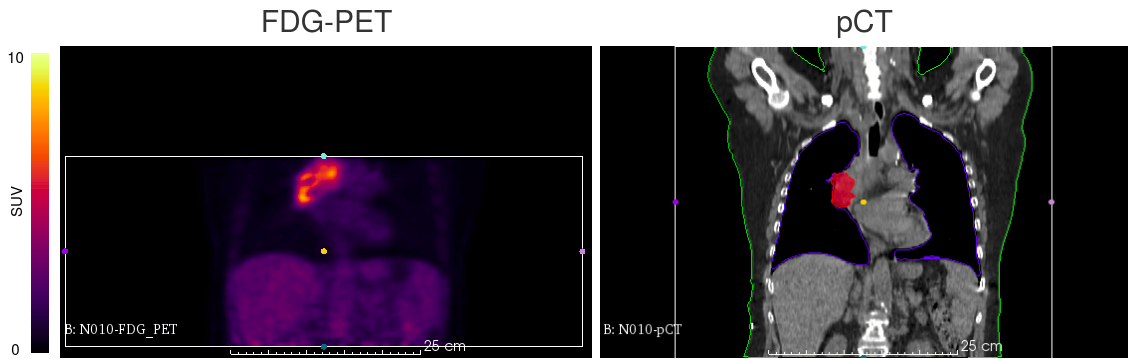
\includegraphics[width=\linewidth]{figures/Data/original/N010-FDG_PET_pCT.png}
    \caption{Single coronal (\textit{x}-\textit{z} plane) slice of FDG-PET and pCT images. White bounding boxes show their respective FOVs. Radiotherapy structure annotations were provided for pCT of which three are shown here -- the patient's body (green), the lungs (dark blue) and the primary tumor (red). The FDG tracer has high specificity to metabolism, resulting in high contrast near the tumor.}
    \label{fig:original_fdgpet_pct}
\end{figure}

In PET image acquisition, a CT scan is usually acquired in the same session whether or not this scan has a separate role, for example, in treatment planning. First, the CT image shows the underlying anatomy for the PET image to be overlaid on it as a contrast map. Second, the material density information captured in the CT scan is used to apply density correction to the recorded PET intensities. The second set of images in the dataset, therefore, includes for each patient an HX4-PET image as well as its accompanying CT scan, both of which are spatially aligned with each other. This CT was acquired using a low radiation dose and is hereafter referred to as \textit{ldCT}. For each patient, the HX4-PET/ldCT scans were acquired on a different day than their corresponding FDG-PET/pCT scans. Both HX4-PET and ldCT images cover approximately the same FOV of the patient's chest. However, the common FOV covered by the HX4-PET/ldCT couple is more focused on the tumor and is smaller in the axial direction compared to that of the FDG-PET/pCT couple. The HX4-PET images have a resolution of 4$\times$4$\times$4 mm$^3$ and the resolution of ldCT is 1.17$\times$1.17$\times$4 mm$^3$. Figure \ref{fig:original_hx4pet_ldct} shows a visualization of sample HX4-PET and ldCT images.

\begin{figure}[h!]
    \centering
    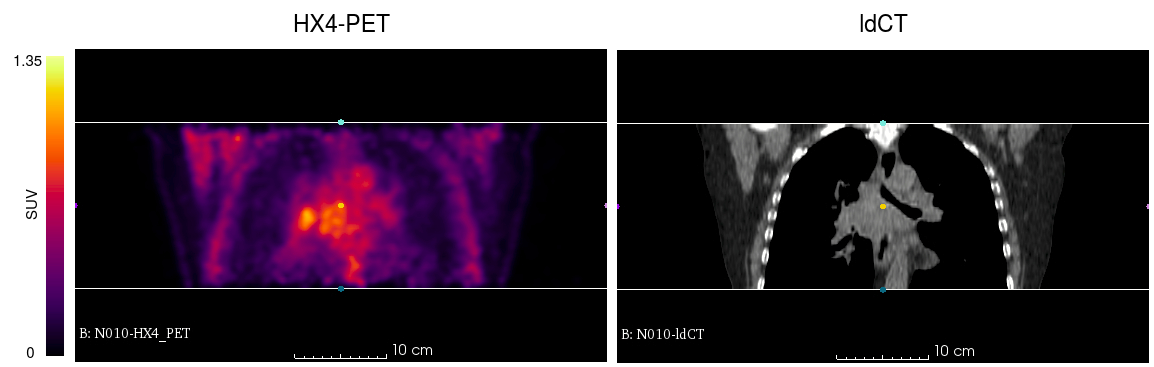
\includegraphics[width=\linewidth]{figures/Data/original/N010-HX4_PET_ldCT.png}
    \caption{Single coronal slice of HX4-PET and ldCT images. Both had similar FOVs. No annotations were provided for the ldCT.}
    \label{fig:original_hx4pet_ldct}
\end{figure}

Voxel intensity values of both pCT and ldCT images are expressed in Hounsfield Units (HU), which relate to the radiodensity of materials. In FDG-PET, the units represent levels of radioactivity emitted from the FDG tracer in different parts of the body as measured by the scanner and are represented in terms of Becquerel per milliliter (Bq/mL, abbreviated as BQML). In HX4-PET, however, intensities are expressed in a different unit called \textit{counts} (abbreviated as CNTS). This unit of PET representation is specific to the manufacturer and the model of the PET/CT scanner (Philips Gemini TF64) that was used for HX4-PET acquisition. Before utilizing the FDG-PET and HX4-PET images for any purpose, their intensities must be converted to a standard and clinically relevant intensity representation -- the Standardized Uptake Value (SUV). SUV calculation is discussed in further detail in \ref{data_proc_phase_1}.


% -----------------------------
\subsection{Image Registration}
Note that the two PET/CT scan pairs -- FDG-PET/pCT and HX4-PET/ldCT -- were acquired on different days for each patient, and because of the differences in patient positioning, they do not spatially align with each other. Having a version of HX4-PET that is aligned with FDG-PET/pCT is essential to serve as the ground truth image for evaluating the GANs as well as for paired training of Pix2Pix. Even et al. \cite{even2017predicting} describe a registration procedure for achieving this alignment. They use a two-step approach where the ldCT is first subjected to rigid alignment followed by non-rigid elastic registration over the pCT. The resulting transformation parameters are then applied to the HX4-PET image.

In addition to the originally acquired scans, the dataset also already includes the registered HX4-PET and ldCT images, and therefore this registration step wasn't needed to be performed. These images are supplied in the \textit{.mhd/.raw} format. The intensity values of the registered HX4-PET are expressed in SUVs, supposedly calculated before the registration process. 

To distinguish the registered HX4-PET from its unregistered counterpart, the two are denoted as \textit{HX4-PET-reg} and \textit{HX4-PET-unreg}, respectively. The term ``HX4-PET" is hereafter used to denote the imaging modality in a general sense and not particularly referring to the registered or unregistered versions of the image. FDG-PET and pCT modalities would be used as inputs to the GAN models and HX4-PET-reg as the ground truth wherever required. Since HX4-PET-reg contains artificial deformations and is likely to contain registration errors as well, the HX4-PET-unreg images instead would be used in the unpaired CycleGAN training. The \textit{unregistered} ldCT, \textit{ldCT-unreg}, would play a crucial role in our modified CycleGAN system, described further in \ref{cyclegan}. However, the \textit{registered} ldCT would not be required anymore beyond this point since its sole purpose was to aid in the registration of HX4-PET, and is thus discarded.


% -------------------------------------
\subsection{Data Preparation Procedure}
\label{Data_Processing}
The dataset needed to be prepared by converting it into a form that could be used for GAN training. The data preparation process can be broken down into two phases, which are elaborated in the following paragraphs. 


\subsubsection{Loading Images and Converting to Appropriate Representation}
The first phase of data preparation involves loading the various images to the computer memory and converting them to a suitable representation. The \textit{PyDicom} library is used for reading the DICOM series along with their metadata, and the \textit{SimpleITK} library for the programmatic representation and manipulation for the loaded images. In certain specialized processing tasks, such as PET SUV calculation and RTstruct conversion, parts of code from this \footnote{HECKTOR 2020 Challenge repository: \url{https://github.com/voreille/hecktor}. It contains utility code created as part of the HECKTOR PET/CT segmentation challenge \cite{andrearczyk2020overview} by its respective authors.} public repository are used to ensure the correctness of the implementation.  

\vspace{4mm}
\noindent
\textit{SUV Calculation:} First, The FDG-PET and HX4-PET-unreg intensity values are converted into the SUV scale. When the intensity units are expressed as BQML, as with all FDG-PET images here, the patient's body weight as well as imaging parameters including the decay time and the total administered dose of the radiotracer are required to calculate the SUV. Equation \ref{BQML_to_SUV} shows the conversion formula. 
\begin{equation}
    SUV = \frac{BQML * 1000 * Weight}{Dose * 2^{-t/\tau}} 
    \label{BQML_to_SUV}
\end{equation}
where $\frac{1}{2^{-t/\tau}}$ is the decay correction factor at time of acquisition \textit{t}, given the half-life $\tau$ of the radiotracer. The values for the patient's weight, administered dose and decay parameters are stored in the DICOM image series as metadata. 

HX4-PET-unreg images, however, are represented in terms of the non-standard CNTS units here, for reasons discussed earlier in \ref{Original_Scans}. CNTS-to-SUV conversion is performed using the formula implemented here \footnote{Implementation of CNTS-to-SUV conversion from the HECKTOR source code: \url{https://bit.ly/3wbtGgW}}.

\vspace{4mm}
\noindent
\textit{Conversion of RTstruct Contours to Binary Masks:} RTstruct is the format defined in the DICOM standard for storing radiotherapy-related annotations (known as ``radiotherapy structure sets") as a set of contour points. The RTstruct file is stored separately from the scans. Since the pCT is used for annotating these contours during radiotherapy treatment planning, the physical coordinate system of the pCT scan is the reference frame for the contour points. Of all the different objects annotated in the pCT scan, we select only the contours for the primary tumor and the patient's body, and convert them to binary masks. Each of these resulting masks has the same 3D size and resolution as the pCT image. The tumor mask would be needed during the clinical evaluation of the hypoxia maps predicted by the models, whereas the body mask would be required during model training to mask away and remove out-of-body objects that are visible in the scans, for instance, the scanner table. The algorithm used for RTstruct-to-binary-mask conversion can be found here \footnote{Implementation of RTstruct-to-binary mask conversion from the HECKTOR source code: \url{https://bit.ly/2RnNI9t}}.

\begin{figure}[h!]
    \centering
    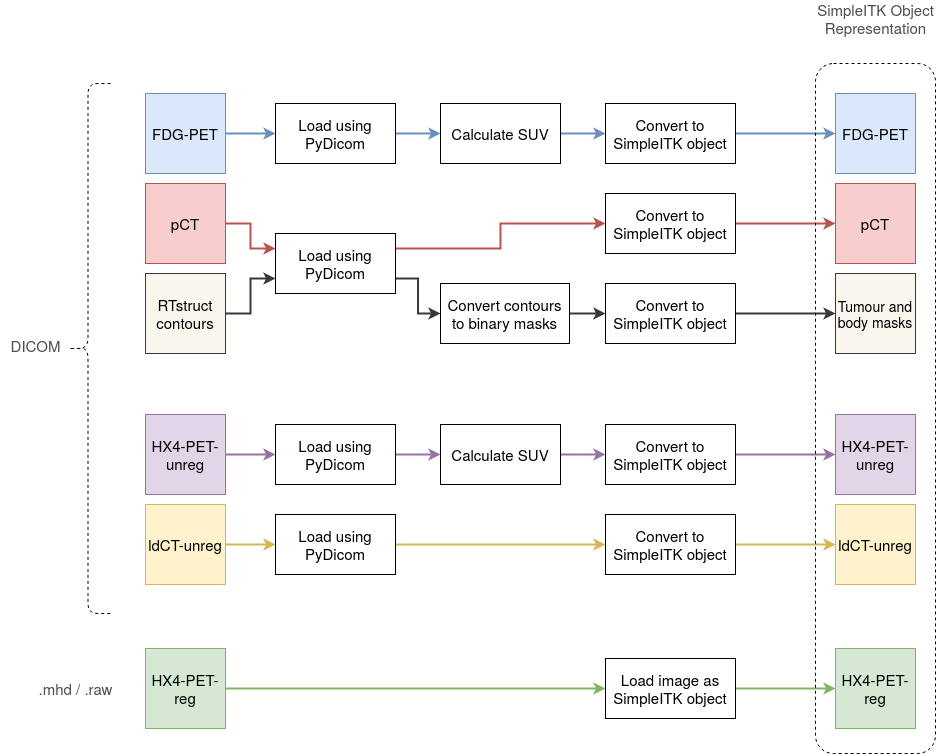
\includegraphics[width=0.9\linewidth]{figures/Data/data_processing_overview-step_1.png}
    \caption{Overview of the first phase of data processing. Images are loaded from storage and converted into a suitable representation for further processing.}
    \label{fig:data_proc_overview_1}
\end{figure}

Following this, the FDG-PET, HX4-PET-unreg, pCT and the tumor and body masks are converted to SimpleITK objects in Python. The ldCT-unreg is also loaded using PyDicom and converted to this representation. HX4-PET-reg, stored in \textit{.mhd/.raw} format containing pre-computed SUV values, is directly loaded into a SimpleITK object. Figure \ref{fig:data_proc_overview_1} shows a visual overview of these steps.


\subsubsection{Cropping and Resampling}
\begin{figure}[h!]
    \centering
    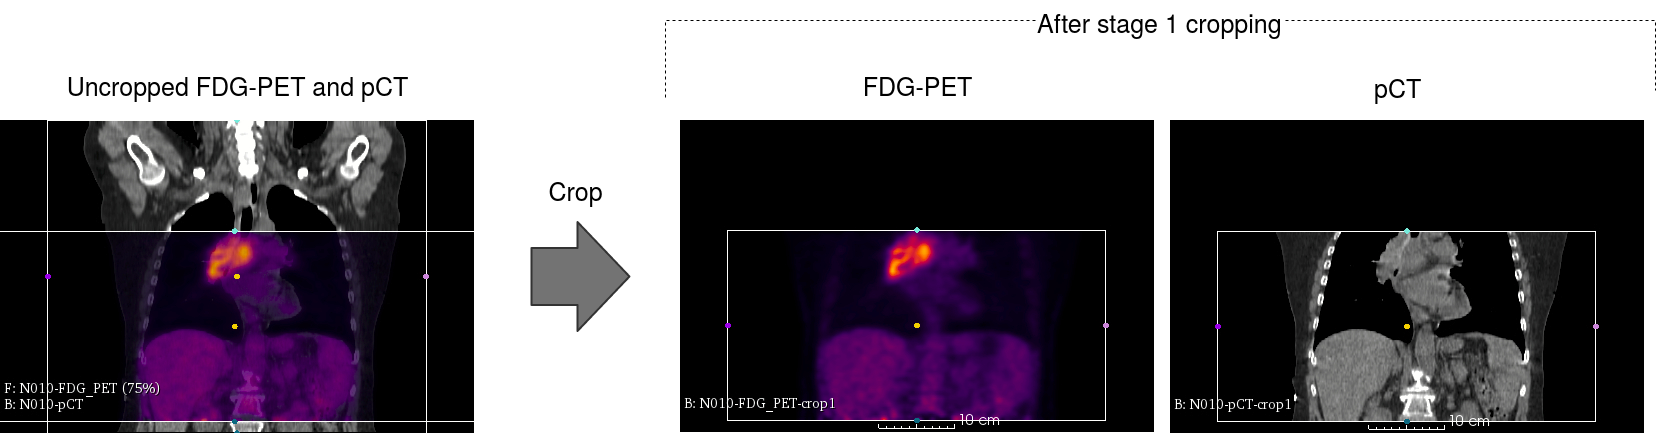
\includegraphics[width=\linewidth]{figures/Data/fdgpet_pct_crop1/N010-FDG_PET_pCT-uncropped_crop1.png}
    \caption{Stage 1 cropping of FDG-PET, pCT and the tumor and body masks (not shown here) to a common FOV. Uncropped FDG-PET and pCT are overlaid to show the overlap of their FOVs.}
    \label{fig:fdg_pet_pct_crop1}
\end{figure}

\begin{figure}[h!]
    \centering
    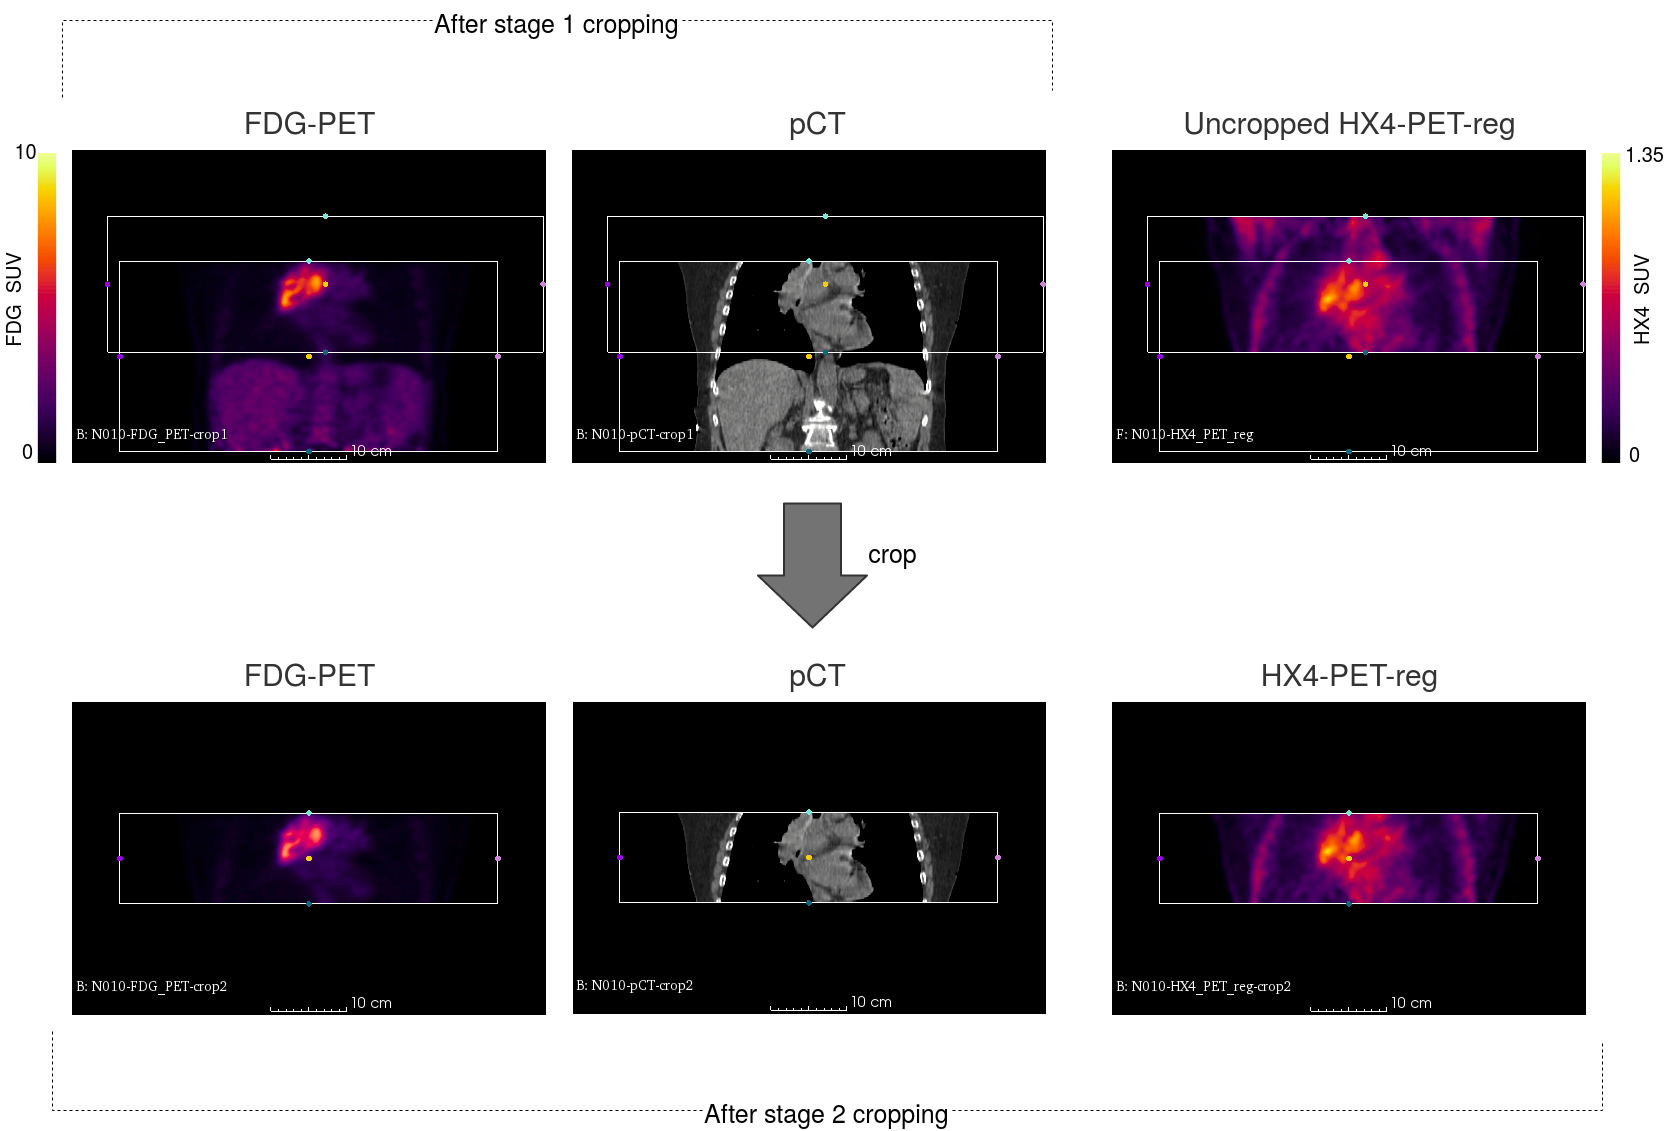
\includegraphics[width=\linewidth]{figures/Data/fdgpet_pct_hx4petreg_crop2/N010-fdgpet_pct_hx4petreg-uncropped_crop2.png}
    \caption{Stage 2 cropping of the input images (FDG-PET and pCT), the masks (tumor and body, not shown here) and the ground truth (HX4-PET-reg) to a common FOV. All FOVs are displayed to show their overlap.}
    \label{fig:fdgpet_pct_hx4petreg_crop2}
\end{figure}

The second phase of data processing involves cropping and resampling the loaded images. A standard resampling resolution of 1$\times$1$\times$3 mm$^3$ is used. Cropping is performed in a progressive manner as described in the following steps: 

\begin{enumerate}
    \item \textit{Cropping and resampling FDG-PET, pCT and masks:} As shown earlier in \ref{Original_Scans}, the FOVs of FDG-PET and pCT are different. Both images must be cropped such that each of them would contain the same FOV of the patient. This is accomplished by determining the 3D volumetric intersection of their FOVs and then cropping the images to this 3D bounding box. Resampling is performed immediately following this. The tumor and body masks share the same FOV with pCT, and are, therefore, cropped in the same way as pCT. This step corresponds to the \textit{Stage 1} cropping of FDG-PET, pCT and the masks. Figure \ref{fig:fdg_pet_pct_crop1} illustrates this step.

    \item \textit{Cropping and resampling HX4-PET-unreg and ldCT-unreg:} The same process of cropping to common FOV followed by resampling is performed on HX4-PET-unreg and ldCT-unreg images. This corresponds to the \textit{Stage 1} cropping of HX4-PET-unreg and ldCT-unreg.

    \item \textit{Resampling HX4-PET-reg:} The HX4-PET-reg image is then only resampled to the standard resolution.

    \item \textit{Cropping the input images, the masks and the ground truth image to common FOV:} Furthermore, the two input images (FDG-PET and pCT), the two masks, and the ground truth image (HX4-PET-reg) are cropped to the common FOV shared across them. The is required because although HX4-PET-reg is spatially aligned with the input images and shares the same physical reference frame with them (due to registration), its FOV is different. This step corresponds to the \textit{Stage 2} cropping, and is visualized in Figure \ref{fig:fdgpet_pct_hx4petreg_crop2}.
\end{enumerate}

\begin{figure}[h!]
    \centering
    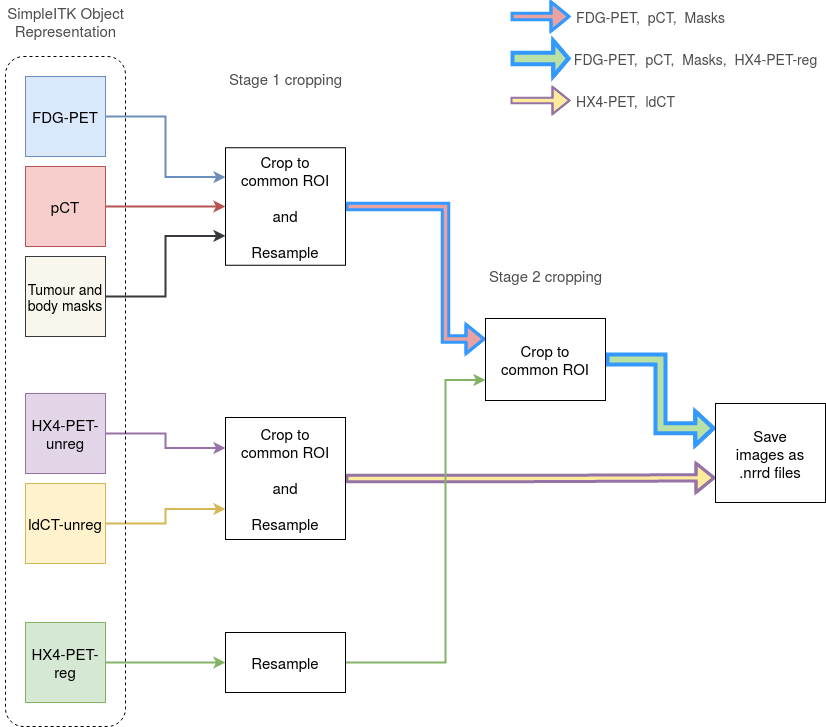
\includegraphics[width=0.8\linewidth]{figures/Data/data_processing_overview-step_2.png}
    \caption{Overview of the second phase of data processing.}
    \label{fig:data_proc_overview_2}
\end{figure}

Finally, all the processed images are saved as \textit{.nrrd} files. The NRRD format allows the storage of N-dimensional raster images along with their spatial information, including voxel spacing (resolution) and physical coordinates of the origin, in a single file. Figure \ref{fig:data_proc_overview_2} shows an overview of the second phase of data processing discussed thus far. The dataset is then split into a training set and a validation set. The training set is comprised of data from the \textit{PET-Boost} clinical trial (15 patients), and the validation set consists of data from the \textit{Nitroglycerin} trial (19 patients). 



%%%%%%%%%%%%%%%%%%%%%%%%%%%%%%%%%%%%%%%%%%%%%%%%%%%%%%%%%%%%%%%%%%%%%%%%%%%%%%%%%%%%%%%%%%%%%%%%%%%%%%%%%%%%%%%%%%%%%%%%%%%%%%%%%%%%%%%%%%%%%%%
\section{GAN Systems}
\label{GAN_Systems}
This section describes the image translation GAN systems used in our study. Unless explicitly mentioned otherwise, domain \textit{A} is used throughout this section to denote the domain of valid multimodal FDG-PET/pCT images, and \textit{B} to denote the domain of HX4-PET images. Synthetic HX4-PET is referred to as \textit{HX4-PET-syn}.


% ------------------
\subsection{Pix2Pix}
\label{pix2pix}
The Pix2Pix framework provides a straightforward image translation method, provided that the domain \textit{A} and domain \textit{B} images in the training dataset are paired, i.e. they are spatially aligned and have pixel-wise correspondence. Given a task of translating a domain \textit{A} image to its equivalent domain \textit{B} image, it is first assumed that an \textit{A}$\rightarrow$\textit{B} mapping exists. The generator models this relationship between the domains, and the discriminator models the conditional probability that an image belongs to domain \textit{B}, given its domain \textit{A} counterpart. During training, the conditional discriminator evaluates the generated domain \textit{B} images, and its adversarial feedback is used to improve the generator's performance. Additionally, Pix2Pix includes an element-wise loss to directly enforce similarity between the synthetic and the ground truth domain \textit{B} images. For a generator $G$ and a discriminator $D$, Equations \ref{eq:pix2pix_loss_components} show the components of each of their loss functions. 

\begin{equation}
    \begin{aligned}
    L(G) &= L_{adv}(G) + \lambda_{elem} L_{elem}(G) \\
    L(D) &= L_{adv}(D)
    \end{aligned}
    \label{eq:pix2pix_loss_components}
\end{equation}
The generator loss has two terms -- an adversarial loss $L_{adv}(G)$ and an element-wise loss $L_{elem}(G)$. The discriminator loss is a single adversarial loss $L_{adv}(D)$ which is the adversarial counterpart of $L_{adv}(G)$. For the generator, $L_{adv}(G)$ can be viewed as a ``structured" loss that is learned from the data itself as a result of the adversarial setting and can produce images with sharp and fine structures, whereas $L_{elem}(G)$ emphasizes on the fidelity of larger and lower-frequency components of the images. The hyperparameter $\lambda_{elem}$ can be used to adjust the balance of importance between the two terms depending on the specific application.

We use the least-squares version of the adversarial loss, instead of the original cross-entropy loss, as it is known to improve training stability \cite{mao2017least}. Similar to the original Pix2Pix framework \cite{isola2017image}, we implement $L_{elem}(G)$ using voxel-wise L1 loss. Equations \ref{eq:pix2pix_loss_expansion} show the expansion of each of these loss terms.

\begin{equation}
    \begin{aligned}
    L_{adv}(G) &= E_{x \sim p_{data}(x)} [(1 - D(x, G(x)))^2]  \\
    L_{adv}(D) &= E_{x \sim p_{data}(x)} [D(x, G(x))^2] + E_{x,y \sim p_{data}(x,y)} [(1 - D(x,y))^2] \\
    L_{elem}(G) &= E_{x,y \sim p_{data}(x,y)} [|| y - G(x) ||_1]  \\
    \end{aligned}
    \label{eq:pix2pix_loss_expansion}
\end{equation}

where $x$ and $y$ are random variables representing paired samples from domain \textit{A} and \textit{B}, respectively. During training, $G$ and $D$ are updated in an alternating fashion. For a given $D$, $G$ learns to synthesize images that $D$ would wrongly classify as real data samples, with value 1 (optimizing for $L_{adv}(G)$), while simultaneously aiming for voxel-wise fidelity of its output with the ground truth (optimizing for $L_{elem}(G)$). Whereas, for a given $G$, $D$ learns to correctly classify the synthetic samples as 0 and the real samples as 1 (thereby optimizing for $L_{adv}(D)$).

\begin{figure}[h!]
    \centering
    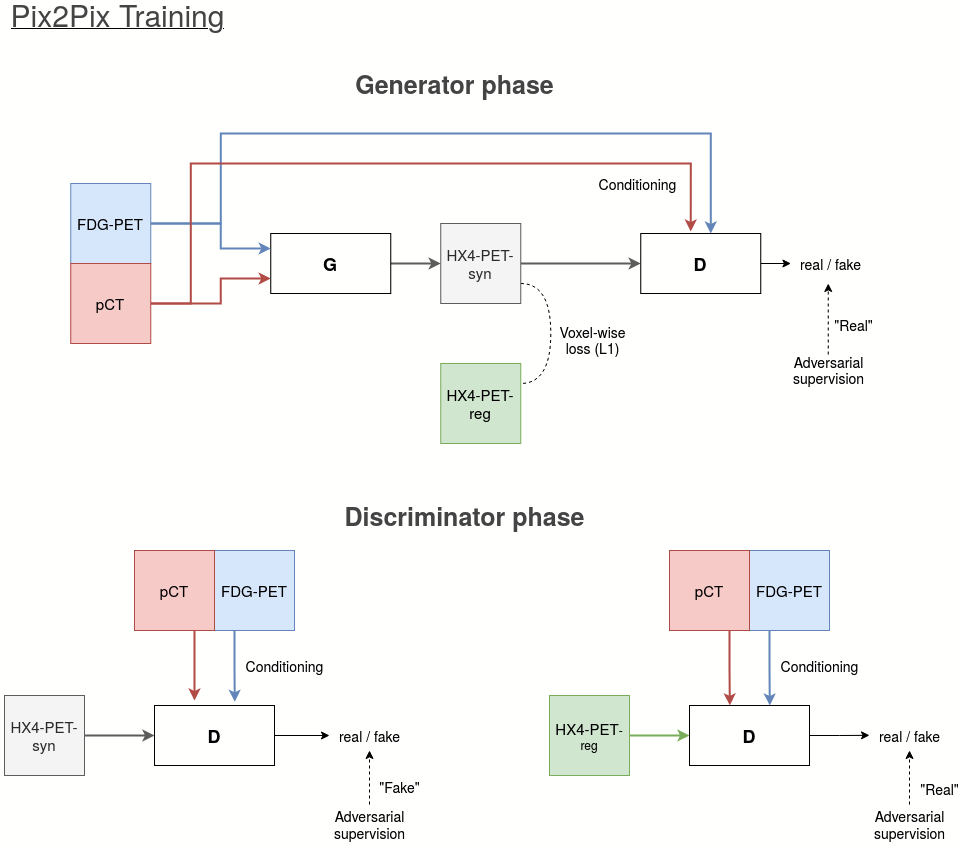
\includegraphics[width=0.9\linewidth]{figures/GANs/Pix2Pix.png}
    \caption{Pix2Pix training phases. \textit{G} and \textit{D} are updated in an alternating manner. In practice, FDG-PET and pCT images are stacked channel-wise and given as input to \textit{G}. And the discriminator conditioning is implemented by stacking channel-wise the HX4-PET-reg or HX4-PET-syn with FDG-PET and pCT.}
    \label{fig:pix2pix}
\end{figure}{}

We apply Pix2Pix to our translation problem in a 3D manner on the volumetric medical images. Given the FDG-PET and pCT images as input and the corresponding HX4-PET-reg images as the target, the model is trained to generate HX4-PET-syn images representative of the target domain. Figure \ref{fig:pix2pix} shows a schematic of the generator and discriminator training phases.


% -------------------
\subsection{CycleGAN}
\label{cyclegan}

CycleGAN addresses unpaired image translation problems where \textit{A}-\textit{B} image pairs are not provided in the training set. It is first assumed that there exists some relationship between domain \textit{A} and domain \textit{B} and that this relationship is bijective in nature. In other words, for an \textit{A}$\rightarrow$\textit{B} transformation, an inverse \textit{B}$\rightarrow$\textit{A} transformation exists. CycleGAN aims at modeling these two mappings simultaneously by incorporating cycle-consistency with the principal idea being that translating an image to another domain and then back to its original domain should yield the same image.  The GAN system consists of two generators -- $G_{AB}$ and $G_{BA}$ -- that implement the \textit{A}$\rightarrow$\textit{B} and \textit{B}$\rightarrow$\textit{A} mappings, respectively. Two discriminators $D_B$ and $D_A$ are adversarially coupled with the respective two generators. Note that, unlike Pix2Pix, discriminators in CycleGAN are not conditioned on input images as this is not possible with unpaired training data. Equations \ref{eq:cyclegan_naive_loss_components} show the generator and discriminator loss terms.

\begin{equation}
    \begin{aligned}
    L(G_{AB}, G_{BA}) &= L_{adv}(G_{AB}) + L_{adv}(G_{BA}) + \lambda_{cyc} L_{cyc}(G_{AB}, G_{BA}) \\[1mm]
    L(D_B, D_A) &= L_{adv}(D_B) + L_{adv}(D_A)
    \end{aligned}
    \label{eq:cyclegan_naive_loss_components}
\end{equation}
The adversarial loss term $L_{adv}(G_{AB})$ of $G_{AB}$ is coupled with $L_{adv}(D_B)$ of $D_B$ and encourages $G_{AB}$ to produce images resembling domain \textit{B} samples. Similarly, $L_{adv}(G_{BA})$ and $L_{adv}(D_A)$ are counterparts of each other and drive $G_{BA}$ to produce images indistinguishable from domain \textit{A}. It would be possible for a generator to satisfy its adversarial constraints by translating its input image from its source domain to just \textit{any} image that would seem like a sample from its target domain, whether or not the translated image preserves the contents of the input image. The cycle-consistency term $L_{cyc}(G_{AB}, G_{BA})$, therefore, acts as an indirect content-preservation criterion that constrains $G_{AB}$ and $G_{BA}$ to preserve the high-level structure across translation, thereby complementing the adversarial losses. The hyperparameter $\lambda_{cyc}$ is used to adjust the relative importance given to cycle-consistency loss. 

Let $x \sim p_{data}(x)$ represent the random variable associated with domain \textit{A} following a distribution $p_{data}(x)$, and $y \sim p_{data}(y)$ be the random variable associated with the domain \textit{B} distribution. Equations \ref{eq:cyclegan_naive_loss_expansion} show each of the loss terms in expanded form.
\begin{equation}
    \begin{aligned}
    L_{adv}(G_{AB}) &= E_{x \sim p_{data}(x)} [(1 - D_B(G_{AB}(x)))^2]  \\[1mm]
    L_{adv}(D_B) &= E_{x \sim p_{data}(x)} [D_B(G_{AB}(x))^2] + E_{y \sim p_{data}(y)} [(1 - D_B(y))^2] \\[4mm]
    L_{adv}(G_{BA}) &= E_{y \sim p_{data}(y)} [(1 - D_A(G_{BA}(y)))^2]  \\[1mm]
    L_{adv}(D_A) &= E_{y \sim p_{data}(y)} [D_A(G_{BA}(y))^2] + E_{x \sim p_{data}(x)} [(1 - D_A(x))^2] \\[4mm]
    L_{cyc}(G_{AB}, G_{BA}) &= E_{x \sim p_{data}(x)} [|| x - G_{BA}(G_{AB}(x)) ||_1]  \\
                            &+ E_{y \sim p_{data}(y)} [|| y - G_{AB}(G_{BA}(y)) ||_1] 
    \end{aligned}
    \label{eq:cyclegan_naive_loss_expansion}
\end{equation}
Cycle-consistency loss $L_{cyc}(G_{AB}, G_{BA})$ encourages a reconstructed image to be as close as possible to its original image in L1 sense, and is applied to both \textit{A}$\rightarrow$\textit{B}$\rightarrow$\textit{A} and \textit{B}$\rightarrow$\textit{A}$\rightarrow$\textit{B} cycles. Figure \ref{fig:cyclegan_concept} shows a conceptual visualization of CycleGAN training.

\begin{figure}
    \centering
    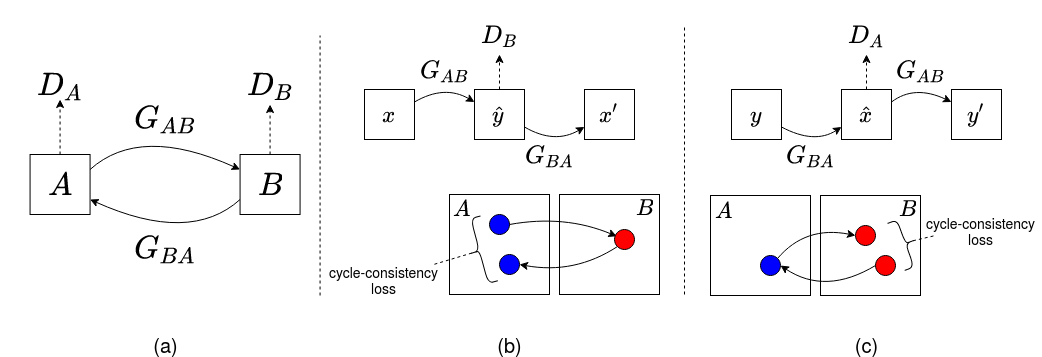
\includegraphics[width=\textwidth]{figures/GANs/cyclegan_concept.png}
    \caption{Simplified representation of CycleGAN training, figure adapted from the original paper \cite{zhu2017unpaired} with notations changed. (a) $G_{AB}$ models \textit{A}$\rightarrow$\textit{B} mapping and $G_{BA}$ its inverse. $D_B$ and $D_A$ are domain \textit{B} and \textit{A} discriminators, respectively. (b) In the \textit{A}$\rightarrow$\textit{B}$\rightarrow$\textit{A} cycle, a domain \textit{A} image $x$ is translated to a representation \textit{$\hat{y} = G_{AB}(x)$} in domain \textit{B}, which is evaluated by $D_B$. It is then used to obtain a reconstruction $x' = G_{BA}(G_{AB}(x))$ of the original image $x$ which is encouraged by the cycle-consistency to be close to $x$. (c) The \textit{B}$\rightarrow$\textit{A}$\rightarrow$\textit{B} cycle.}
    \label{fig:cyclegan_concept}
\end{figure}


\subsubsection{CycleGAN-naive: Default CycleGAN applied to HX4-PET synthesis problem}
We investigate CycleGAN for unpaired translation of FDG-PET/pCT to HX4-PET. The term ``unpaired" can be used at two levels here -- the patient level and the voxel level. At the patient level, our dataset includes all three image modalities for each patient. The training data used for the CycleGAN is patient-level unpaired, meaning the \textit{A}-\textit{B} image correspondence information is not used, and both domain \textit{A} and domain \textit{B} samples are independently shuffled while training. At the voxel level, the registered HX4-PET-reg images are spatially aligned input-target paired data, whereas the unregistered images -- HX4-PET-unreg -- are devoid of any artificial deformations and imperfections that are related to registration. We, therefore, use HX4-PET-unreg images as the set of domain \textit{B} samples which results in our CycleGAN training data being unpaired at the voxel level as well. The default CycleGAN framework naively applied to our use case is henceforth referred to as \textit{CycleGAN-naive}. Figure \ref{fig:cyclegan_naive} shows a schematic of the generator and discriminator training phases of CycleGAN-naive. 

\begin{figure}[h!]
    \centering
    \makebox[\textwidth][c]
    {
        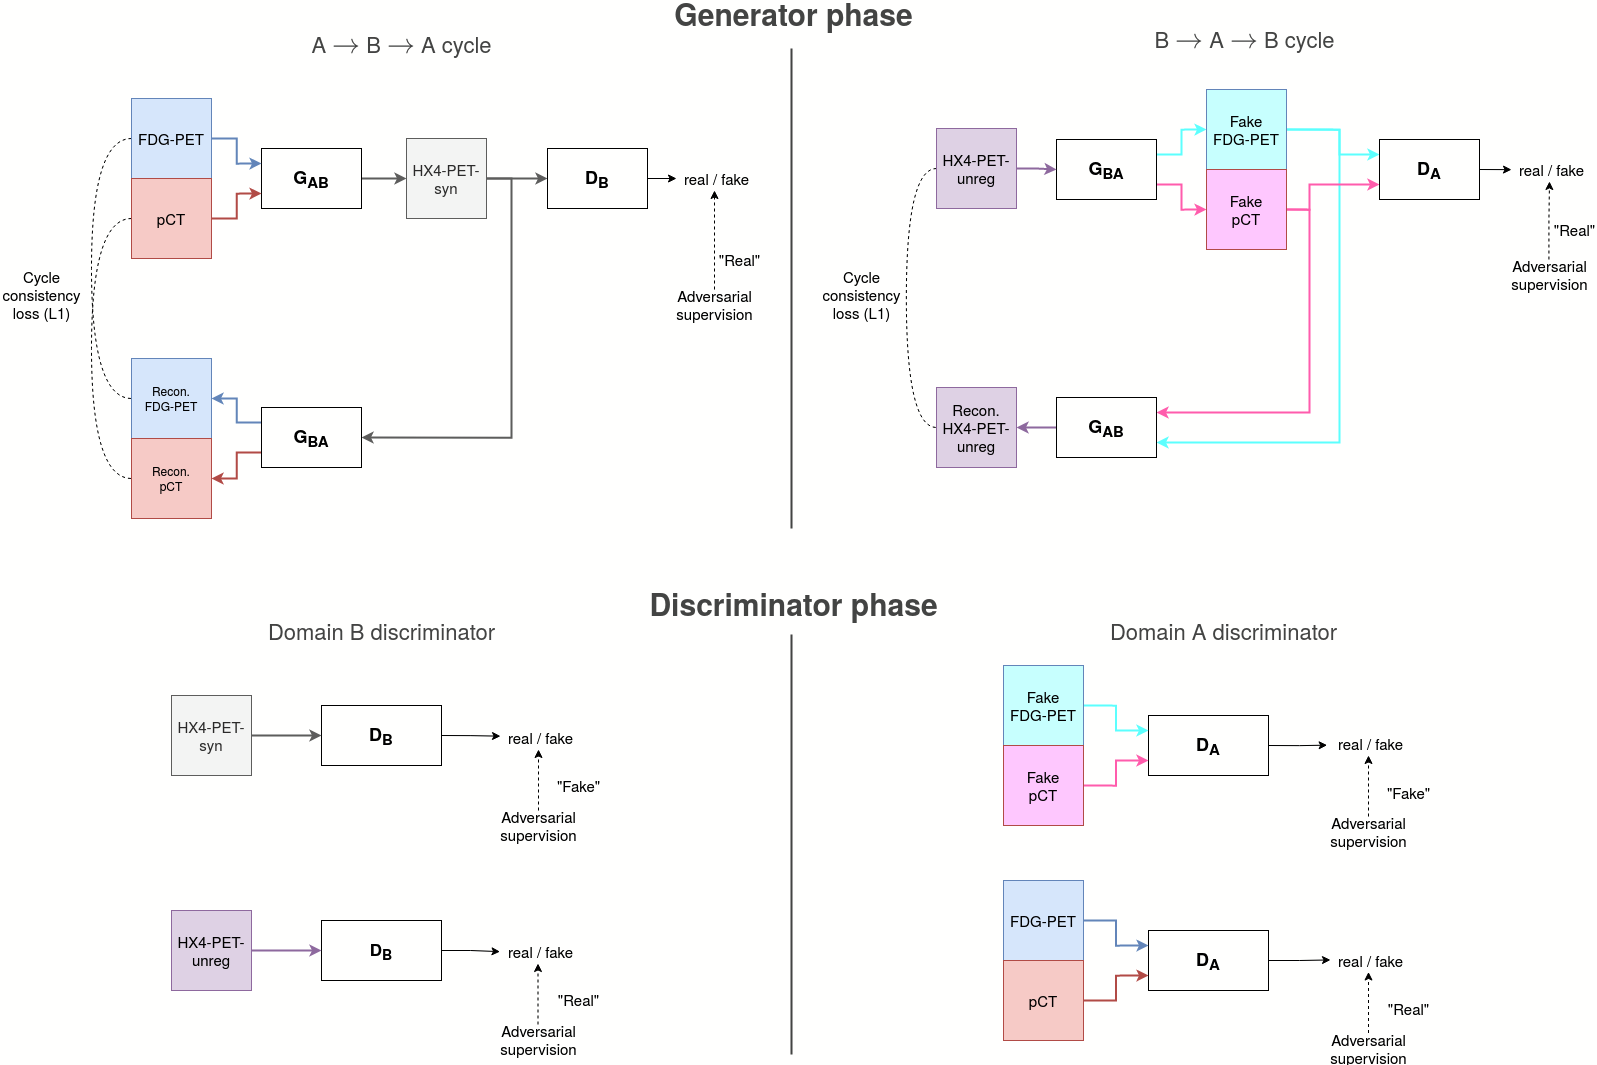
\includegraphics[width=1.5\linewidth]{figures/GANs/CycleGAN-naive.png}
    }
    \caption{CycleGAN-naive training phases. The generators and discriminators are updated in an alternating manner.}
    \label{fig:cyclegan_naive}
\end{figure}{}

We argue that CycleGAN-naive has several drawbacks and therefore, it is not an optimal implementation of CycleGAN for our task. In the \textit{A}$\rightarrow$\textit{B}$\rightarrow$\textit{A} cycle, $G_{AB}$ takes as input FDG-PET and pCT to output HX4-PET-syn, and $G_{BA}$ uses HX4-PET-syn to reconstruct FDG-PET and pCT. The learning task of $G_{AB}$ is realistic since hypoxia patterns can be reliably predicted from the inputs, and therefore, has a physiological basis (see Section \ref{Related_Work-hypoxia_prediction}). However, the learning task of $G_{BA}$ is not reasonable. It is not possible to precisely predict a patient's anatomy (CT) as well as their metabolism levels (FDG-PET) from just the hypoxia information, and the CT modality is of more concern to our discussion. A CT image contains highly detailed structural information with sharp and fine features, whereas PET images are functional heatmaps having blurred and diffused characteristics. $G_{BA}$ cannot accurately rebuild pCT from HX4-PET-syn unless $G_{AB}$ encodes the CT information into the latter in the form of noise. But then, the HX4-PET-syn image would not resemble a clinically acquired HX4-PET scan. Therefore, cycle-consistency constraint conflicts with the domain \textit{B} adversarial criterion instead of complementing it. Now looking at the \textit{B}$\rightarrow$\textit{A}$\rightarrow$\textit{B} cycle, the task of $G_{BA}$ is to compute realistic FDG-PET and pCT when given only the real HX4-PET-unreg image, which it can perform, especially for pCT, by hallucinating the patient's anatomy. However, in that case, $G_{AB}$ would be given this fake information to precisely reconstruct the HX4-PET-unreg. Because the task of $G_{AB}$ is to correctly predict hypoxia based on given CT (and FDG-PET) information, it is unreasonable to provide it with fake anatomical information and expect it to predict hypoxia patterns from it that match the real HX4-PET-unreg. Hence, in this cycle as well, cycle-consistency requirement conflicts with the adversarial objective. The fundamental assumption made by CycleGAN regarding the existence of a bijective relationship between domains \textit{A} and \textit{B}  does not hold here, and the resulting images are likely to be highly inaccurate and not representative of the patient's condition. Based on these reasons, we believe that CycleGAN, in its default form, cannot tackle this translation problem and that a more intelligent strategy is required.


\subsubsection{CycleGAN-balanced: An improved design}
We propose a custom design improvement to CycleGAN training to make the system more optimized for our use case. We utilize the fact that an HX4-PET scan is always acquired together with a CT scan which, in our dataset, is a low-dose CT (ldCT). Model training is unpaired similar to CycleGAN-naive, and the ldCT-unreg images are included in the training data accompanying their corresponding HX4-PET-unreg images. 

We begin by slightly altering what the domains \textit{A} and \textit{B} denote here -- let \textit{A} be the domain of FDG-PET images and \textit{B} of HX4-PET images. The CT images -- pCT and ldCT -- are then considered to be ``supporting" images that provide \textit{anatomical context} to the generators. Note that pCT has spatial correspondence only with FDG-PET, and ldCT-unreg is aligned only with HX4-PET-unreg. Now, the task of each generator is to take as input a PET image from its source domain and compute its target domain PET image, while being supplied anatomical context using the \textit{available} CT image (i.e the one that is aligned with the source domain PET). To elaborate on this, consider the two cycles separately: 

\begin{itemize}
    \item \textit{A$\rightarrow$B$\rightarrow$A cycle}: Here, pCT is the available CT image which accompanies the FDG-PET. In \textit{A}$\rightarrow$\textit{B} translation, $G_{AB}$ uses the two images and computes HX4-PET-syn. In \textit{B}$\rightarrow$\textit{A} translation, $G_{BA}$ now \textit{reuses} the pCT as a support image along with the HX4-PET-syn (note that the two are aligned) to reconstruct FDG-PET. The pCT provides the same anatomical context for FDG-PET reconstruction as it did for HX4-PET-syn prediction. The cycle-consistency loss is computed between the FDG-PET and its reconstructed version. If the HX4-PET-syn represents a plausible hypoxia prediction, then the FDG-PET can be recovered from it up to a great extent since both have an underlying physiological relationship. Therefore, the adversarial loss would drive $G_{AB}$ to produce realistic HX4-PET-syn image and the cycle-consistency loss would encourage this image to be representative of the patient's physiology. 
    
    \item \textit{B$\rightarrow$A$\rightarrow$B cycle}: In this case, ldCT-unreg is the available CT image that is coupled with the HX4-PET-unreg. In \textit{B}$\rightarrow$\textit{A} translation, $G_{BA}$ uses these two images to compute a synthetic FDG-PET. In \textit{A}$\rightarrow$\textit{B} translation, $G_{AB}$ reuses the ldCT-unreg and together with the synthetic FDG-PET (note that the ldCT-unreg and the synthetic FDG-PET are aligned), it reconstructs HX4-PET-unreg. Cycle-consistency is applied between the original and reconstructed HX4-PET-unreg. The same ldCT-unreg image provides anatomical context for FDG-PET synthesis and for HX4-PET-unreg reconstruction, and if the synthetic FDG-PET represents plausible metabolism patterns, then HX4-PET-unreg can be mostly recovered. In this cycle as well, the adversarial and cycle-consistency objectives would behave in a mutually reinforcing manner.
\end{itemize}

The introduction of CT as an \textit{input} to both the generators creates a balance between the complexities of the \textit{A}$\rightarrow$\textit{B} and \textit{B}$\rightarrow$\textit{A} mappings since none of them involves \textit{predicting} fake CT information, while still using completely unpaired training data. Unlike CycleGAN-naive, the \textit{A}$\rightarrow$\textit{B} and \textit{B}$\rightarrow$\textit{A} relations are not anymore inverses of each other, in the strict sense of the word. We term this modified design \textit{CycleGAN-balanced}. Figure \ref{fig:cyclegan_balanced} shows a schematic of the training phases of its generators and discriminators.

\begin{figure}[h!]
    \centering
    \makebox[\textwidth][c]
    {
        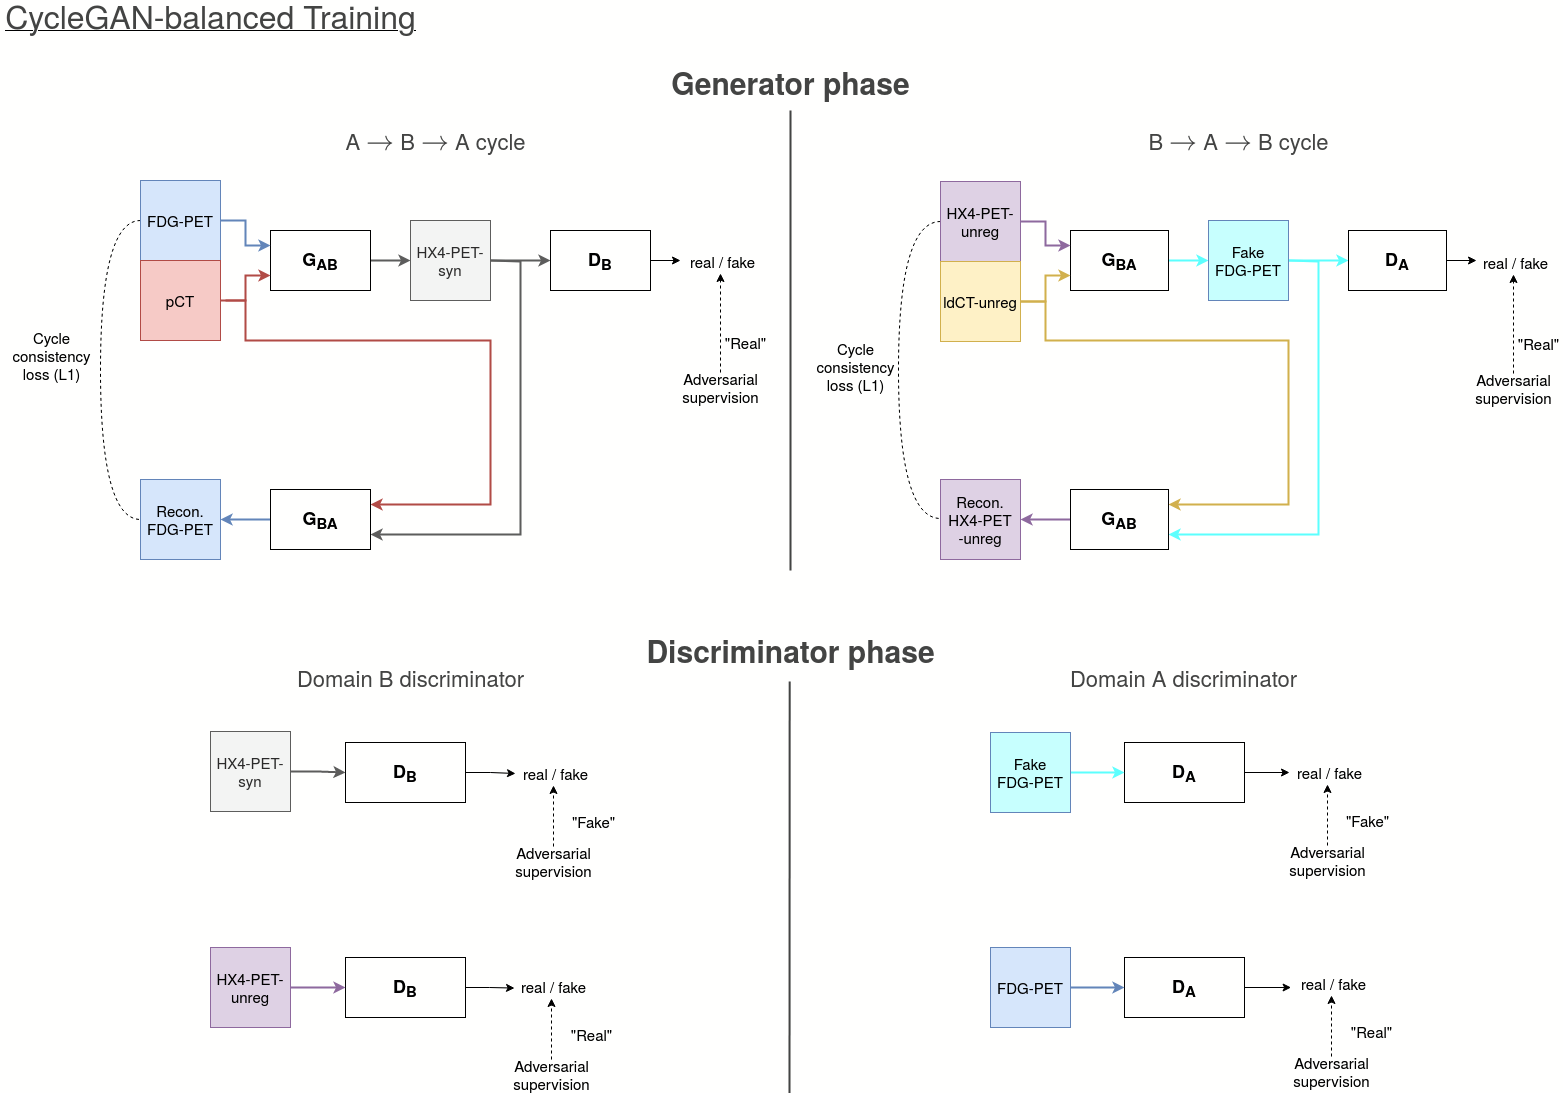
\includegraphics[width=1.5\linewidth]{figures/GANs/CycleGAN-balanced.png}
    }
    \caption{CycleGAN-balanced training phases. \textit{A}$\rightarrow$\textit{B} and \textit{B}$\rightarrow$\textit{A} translation tasks are balanced. The CT images provide anatomical context to the generators. In \textit{A}$\rightarrow$\textit{B}$\rightarrow$\textit{A} cycle, the pCT is used as an input by $G_{AB}$ and then reused by $G_{BA}$. In the \textit{B}$\rightarrow$\textit{A}$\rightarrow$\textit{B} cycle, the ldCT-unreg is the common CT image used by both the generators.}
    \label{fig:cyclegan_balanced}
\end{figure}{}

Low-dose CT scans are characterized by a higher amount of acquisition-related noise compared to routine- or high-dose CT scans (such as planning CT). An additional, possibly desirable, consequence of exposing the two generators to both pCT and ldCT images during training is that the model is likely to learn effectively the relevant anatomical features while disregarding any pCT-specific or ldCT-specific noise signatures. That is, they are likely to generalize over both types of CT images. This is merely a property of CycleGAN-balanced that we make a note of, although we do not investigate this further.


%%%%%%%%%%%%%%%%%%%%%%%%%%%%%%%%%%%%%%%%%%%%%%%%%%%%%%%%%%%%%%%%%%%%%%%%%%%%%%%%%%%%%%%%%%%%%%%%%%%%%%%%%%%%%%%%%%%%%%%%%%%%%%%%%%%%%%%%%%%%%%%
\section{Network Architecture}
\label{network_architectures}
The Pix2Pix, CycleGAN-naive, and CycleGAN-balanced systems share the same generator and discriminator network architectures for the sake of fair comparison. Our design choices of the architectures are based on the specifications of the original Pix2Pix and CycleGAN frameworks \cite{isola2017image, zhu2017unpaired} and involve the 3D equivalent of the 2D spatial operations.

% --------------------
\subsection{Generator}
Each generator network is based on the 3D U-Net architecture \cite{cciccek20163d}. 3D U-Net is a fully convolutional network that takes as input a 3D volumetric image of arbitrary size and can produce an output image of the same size as the input. It consists of an \textit{analysis} path (or encoder) where hierarchical features are progressively extracted from the input image and a \textit{synthesis} path (or decoder) that progressively constructs the output image from the features. A desirable property of the U-Net is its skip connections that transport features of multiple abstraction levels directly into the synthesis path, enabling it to utilize both high- and low-level features in synthesizing the output. In contrast to a U-Net, a traditional encoder-decoder network without any skip-connections must depend on its highest-level features (i.e. features from its ``bottleneck" ). In many image translation problems, the input and target domain images could share a large amount of low-level information. The U-Net is known to produce better quality images in such cases compared to the encoder-decoder architecture \cite{isola2017image}.

Loosely based on the notation used in \cite{isola2017image}, we use \textit{Enc-Ck} to represent an encoder block composed of Convolution-InstanceNorm-LeakyReLU layers where the convolution operation uses \textit{k} 3D kernels of size 4$\times$4$\times$4 voxels, applied with a stride 2$\times$2$\times$2 and zero padding of 1 at each side of the input along each axis. The Leaky ReLU has a negative side slope of 0.2. For the decoder, let \textit{Dec-Tk} represent a block comprising of TransposedConvolution-InstanceNorm-ReLU layers where the 3D upsampling transposed convolution uses \textit{k} kernels of size 4$\times$4$\times$4, stride 2$\times$2$\times$2, and input padding of 1 at each side along each axis. With the given configuration, the encoder downscales the image representation by a factor of 2 at every stage, and the decoder upscales it by the same factor. Our U-Net architecture is then specified in Table \ref{tab:generator_architecture}.

\begin{table}[h!]
    \centering
    \begin{tabular}{|c|c|c|}
        \hline
        \textbf{Encoding Level} & \textbf{Encoder block} & \textbf{Decoder block} \\
        \hline
        1     & Enc-C64          & Dec-T1           \\
        \hline
        2     & Enc-C128         & Dec-T64          \\
        \hline
        3     & Enc-C256         & Dec-T128         \\
        \hline
        4     & Enc-C512         & Dec-T256         \\
        \hline
        5     & Enc-C512         & Dec-T512         \\
        \hline
    \end{tabular}
    \caption{The first encoder block Enc-C64 accepts a two-channel input image and the encoder path processes the image from encoding level 1 to 5. The first decoder block Dec-T512 is in correspondence with the last encoder block Enc-C512, and the decoder path performs computation starting from encoding level 5 to 1, ultimately producing a single channel output image from Dec-T1. An exception to the U-Net's input and output channels appears in CycleGAN-naive, where the generator $G_{BA}$ requires a single channel input and produces a two-channel output.}
    \label{tab:generator_architecture}
\end{table}

There are two exceptions to the aforementioned block notations. The first encoder block (Enc-C64) and the last decoder block (Dec-T1) do not use instance normalization. And, the latter uses the \textit{tanh} activation function to output an image with intensity values bounded within the range (-1, 1). 


% ------------------------
\subsection{Discriminator}
We use the 3D PatchGAN architecture for our discriminators. The network is essentially a convolutional classifier that, instead of computing a single validity score for an image (0 if fake, 1 if real), evaluates independent scores for fixed-size local regions (or patches) of the image. It, therefore, encourages the synthetic images to not only resemble the target domain at the global level but also for its local high-frequency structures to reflect the characteristics of the domain. PatchGAN discriminator of a fixed architecture can take an input image of arbitrary size and produces an output map whose size depends on the input image size, while each output unit's \textit{receptive field} size is constant with respect to the input image. The receptive field size can be increased by increasing the depth of the network.

Let \textit{Ck} denote a block composed on Convolution-InstanceNorm-LeakyReLU where the 3D convolution layer uses \textit{k} kernels of size 4$\times$4$\times$4 and input padding of 1 at each side along each axis, and the Leaky ReLU has a negative side slope of 0.2. The exact discriminator architecture is then shown in Table \ref{tab:discriminator_architecture}. Under this configuration, the receptive field of each output unit is 70$\times$70$\times$70 voxels on the input image.

\begin{table}[h!]
    \centering
    \begin{tabular}{|c|c|}
        \hline
        \textbf{Block number} & \textbf{Discriminator block}\\
        \hline
        1     & C64       \\
        \hline
        2     & C128      \\
        \hline
        3     & C256      \\
        \hline 
        4     & C512      \\
        \hline
        5     & C1        \\
        \hline
    \end{tabular}
    \caption{The first discriminator block C64 takes as input a single channel image (except of $D_A$ of CycleGAN-naive which requires two-channel input). The last block C1 always outputs a single-channel validity score map. Blocks 1, 2 and 3 use a stride of 2$\times$2$\times$2 resulting in a downscaling of the image representation by a factor of 2, whereas blocks 4 and 5 uses a stride of 1$\times$1$\times$1.}
    \label{tab:discriminator_architecture}
\end{table}
As exceptions to the notation, instance normalization is not used in the first and the last blocks. Also, because we use the least-squares adversarial loss, the last block does not include an activation function. The final convolution layer's output map is considered the discriminator's final output.



%%%%%%%%%%%%%%%%%%%%%%%%%%%%%%%%%%%%%%%%%%%%%%%%%%%%%%%%%%%%%%%%%%%%%%%%%%%%%%%%%%%%%%%%%%%%%%%%%%%%%%%%%%%%%%%%%%%%%%%%%%%%%%%%%%%%%%%%%%%%%%%
\section{Model Training}


% --------------------------------------------
\subsection{Overview of the Data Requirements}
\label{data_requirements}
Figure \ref{fig:which_images_where} provides a visual overview of the data requirements of each GAN system to clarify which image type is used where, much of which is covered in detail earlier in Section \ref{GAN_Systems} for each individual GAN. The FDG-PET and pCT images comprise the model input. HX4-PET-reg is the ground truth hypoxia map, and images from the validation set are used to evaluate and track model generalizability during the training process. HX4-PET-reg images from the training set are used to train the paired Pix2Pix model. The unregistered image couples HX4-PET-unreg and ldCT-unreg are required only in the training set, of which only the HX4-PET-unreg is involved in CycleGAN-naive training, whereas both are used in CycleGAN-balanced training.

\begin{figure}[h!]
    \centering
    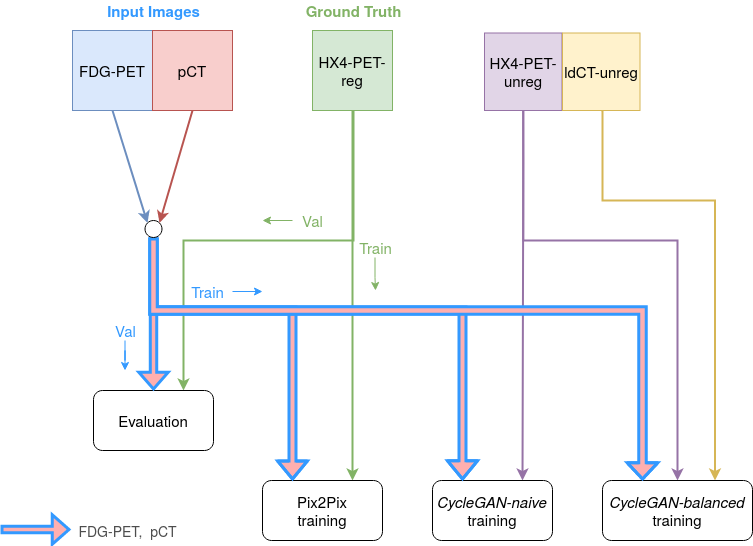
\includegraphics[width=0.8\linewidth]{figures/Data/which_images_where.png}
    \caption{Overview of data requirements of the GAN systems.}
    \label{fig:which_images_where}
\end{figure}


% ----------------------------
\subsection{Training Pipeline}
\label{training_pipeline}

\subsubsection{Data pre-processing and normalization}
Depending on the GAN, the required training images and the body mask are first fetched from their \textit{.nrrd} form into the computer memory. The body mask is applied to pCT, FDG-PET, and HX4-PET-reg (if using), and the out-of-the-body region intensities are set to zero signal value -- i.e. 0 SUV (zero activity) in the PET images and -1024 HU (value for air) in pCT. This body mask was obtained from the pCT (see \ref{Data_Processing}), and therefore, cannot be applied to the unregistered images. When performing unpaired training with HX4-PET-unreg and ldCT-unreg, the latter is used to automatically generate their own body mask via HU thresholding and morphological operations. This new body mask is then applied to HX4-PET-unreg (and ldCT-unreg, if using). Body masking is then followed by normalization. CT intensities are clipped and limited to the HU range [-1000, 2000] and then linearly rescaled to range [-1, 1]. FDG-PET is clipped into the SUV range [0, 15] followed by rescaling to [-1, 1]. In the case of HX4-PET images, following previous related work \cite{even2017predicting}, the SUV values are first divided by the mean SUV of the patient's aorta region. The resulting intensity representation ($\frac{SUV}{SUV_{aorta-mean}}$ ratio) has a special meaning when used in the context of the tumor, wherein it is referred to as the tumor-to-background ratio (TBR). Here, the aorta is considered the ``background" with respect to the tumor. This is a clinically useful intensity representation that has pre-defined standard thresholds \cite{zegers2013hypoxia} and can, hence, be used for hypoxia quantification during image evaluation (described further in Section \ref{Evaluation_Methods}). We perform this conversion step at the beginning of the training pipeline, instead of during the evaluation stage, because the aorta annotation was not provided in the dataset which makes it impossible to compute the $SUV_{aorta-mean}$ value directly from the HX4-PET images. These values were instead provided for each patient directly in a separate file, and we had to depend on them for SUV $\leftrightarrow$ TBR conversion throughout the training and evaluation stages. Following the conversion of the body masked HX4-PET images into this intensity unit, the intensities are clipped to the range [0, 3] and then rescaled to [-1, 1]. The aforementioned clipping ranges for FDG-PET SUV and HX4-PET $\frac{SUV}{SUV_{aorta-mean}}$ are used because they covered most of the intensity variation in their respective images, especially in the tumor area.

\subsubsection{Patch-based training}
We use a patch-based training approach to cope with the high memory requirements of the 3D GANs and with the small size of the training set. For each pre-processed image, a single 3D patch is extracted from the image and is used to feed the model. The body mask is used to limit patch sampling to the body region to avoid extracting patches from the background. Patches from the input images (FDG-PET and pCT) are sampled randomly with a uniform random distribution over the body region. Then, depending on whether the training is paired or unpaired, a suitable \textit{patch propagation} strategy is used to obtain a corresponding patch from the given HX4-PET image.

Let $f_A$ be the location of the focal point of the patch sampled from the input images. During paired training, a corresponding focal point $f_B$ in HX4-PET-reg is then calculated simply as $f_B = f_A$, since this image is spatially aligned to the input images. Figure \ref{fig:paired_patch_sampling} shows a simplified visualization of the paired patch sampling process.

\begin{figure}[h!]
    \centering
    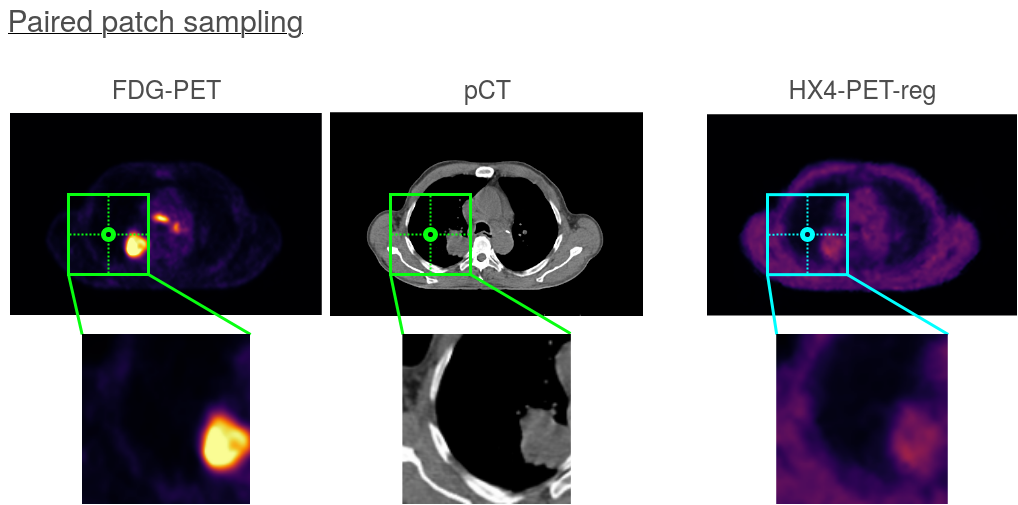
\includegraphics[width=\linewidth]{figures/Data/patch_sampling/paired_patch_sampling.png}
    \caption{Using uniform random sampling in the body region, focal point $f_A$ coordinate (green circles) is first sampled from FDG-PET (and pCT). A corresponding point $f_B$ (cyan circle) is then propagated to HX4-PET-reg such that $f_B = f_A$. Since all three images are spatially aligned, the resulting patches (green and cyan bounding boxes) are aligned as well and cover the same exact anatomical region.}
    \label{fig:paired_patch_sampling}
\end{figure}

In case of unpaired training, a more sensible patch propagation strategy is used instead of sampling patches randomly and independently from the input images and the target domain's unregistered images. The idea is to create a form of ``weak pairing" between the two sets of patches like so -- the anatomical region covered in the input image patches and the HX4-PET-unreg patch should be roughly similar, even though the the input and the target domain images correspond to two different patients. We exploit the fact that all scans have the same patient orientation and a similar FOV. Given the focal point $f_A$ of the patch sampled from the input images, an equivalent focal point $f_B$ is estimated on the HX4-PET-unreg as shown in Equation \ref{eq:unpaired_patch_sampling}.
\begin{equation}
    f_B = \frac{f_A}{size_A} size_B
    \label{eq:unpaired_patch_sampling}
\end{equation}
$f_B$ is calculated such that its relative position with respect to the volume size $size_B$ of the HX4-PET-unreg image is same as the relative position of $f_A$ with respect to the size $size_A$ of the input images. This is then followed by defining a \textit{local sampling region} of size $l_x \times l_y \times l_z$ around $f_B$ and then updating $f_B$ by randomly sampling from this local sampling region. Let this new focal point be denoted as $f_B'$. Again, the condition is applied on $f_B'$ that it must lie within the patient's body region and not in the image background. This additional stochasticity is introduced in the process to account for possible variation in the body position and anatomy across patients. When using ldCT-unreg (i.e. during CycleGAN-balanced training), it shares the same $f_B'$ as HX4-PET-unreg. Figure \ref{fig:unpaired_patch_sampling} shows a visual representation of the unpaired patch sampling process.

\begin{figure}[h!]
    \centering
    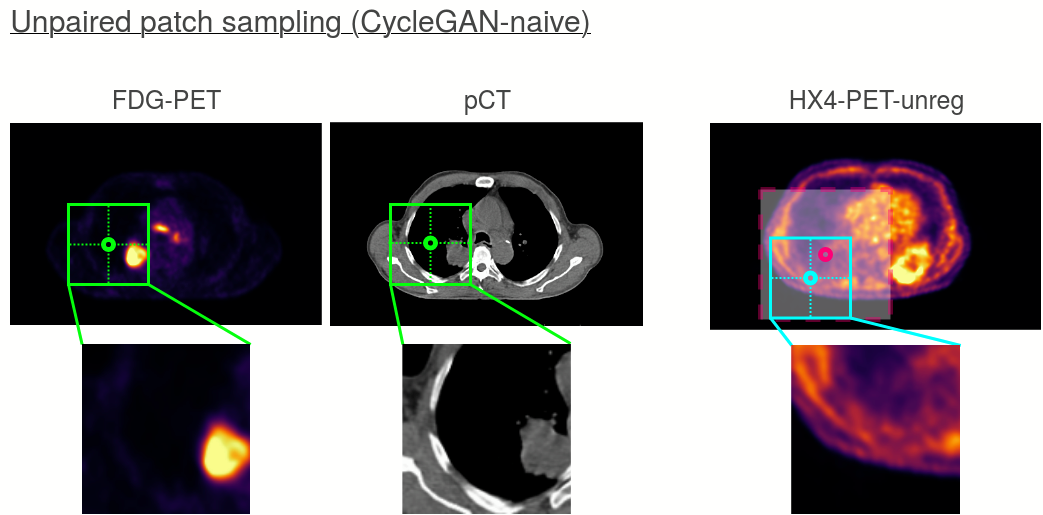
\includegraphics[width=\linewidth]{figures/Data/patch_sampling/unpaired_patch_sampling.png}
    \caption{Given a focal point $f_A$ (green circles) in the input images, a point $f_B$ (pink circle) is propagated to the HX4-PET-unreg image and a local sampling region (pink translucent bounding box) is defined around it. A new point $f_B'$ (cyan circle) is then sampled from this local region and is used to define the HX4-PET-unreg patch (cyan bounding box). Both sets of patches cover similar anatomical regions, despite belonging to images of two different patients.}
    \label{fig:unpaired_patch_sampling}
\end{figure}

The local sampling region is specified as a fraction of the volume size of HX4-PET-unreg image, and in our experiments, we use size 35\% $\times$ 35\% $\times$ 60\%. This relatively large size is set to provide just sufficient freedom for a set of valid patches to be sampled from the full images. A similar, yet much simpler, 2D slice-based unpaired patch sampling was previously suggested by Yang et al. \cite{yang2018unpaired} which produced better results compared to randomly and independently selecting slices for training. We use a fixed patch size of 128$\times$128$\times$32 voxels in both paired and unpaired cases.


\subsubsection{Patch-based validation}
A patch-based inference is used during the model validation phase using a \textit{sliding window} scheme \footnote{Sliding window inferer: \url{https://docs.monai.io/en/latest/inferers.html}}. The same patch size as used in training is used here as well. Given a pair of full-size input images, overlapping patches are sequentially extracted and fed into the GAN model independently. Their corresponding predicted HX4-PET-syn patches are then stitched together into the full-size HX4-PET-syn image. Following this, various image similarity metrics (discussed further in \ref{image_quality_metrics}) are computed between this HX4-PET-syn image and its ground truth HX4-PET-reg. We rescale the predicted and the ground truth images back to their prior intensity scale ($\frac{SUV}{SUV_{aorta-mean}}$ ratio) before computing the metrics. The HX4-PET-syn images are then converted back into SUV intensity representation and saved as NRRD files for later inspection.



%%%%%%%%%%%%%%%%%%%%%%%%%%%%%%%%%%%%%%%%%%%%%%%%%%%%%%%%%%%%%%%%%%%%%%%%%%%%%%%%%%%%%%%%%%%%%%%%%%%%%%%%%%%%%%%%%%%%%%%%%%%%%%%%%%%%%%%%%%%%%%%
\section{Evaluation Methods}
\label{Evaluation_Methods}
The validation set used to track model generalizability is the same data used for final evaluation. We perform an evaluation on the predicted HX4-PET-syn from two different perspectives. In the first, the objective is to evaluate the overall success of the models in learning the input-target mapping, and the evaluation is performed by assessing the fidelity of the full synthetic samples produced by the models with respect to the ground truth. The second perspective regards the clinical value of the synthetic hypoxia maps as the most important factor since the clinical utility of the models is the end goal. In a clinical scenario, the tumor is the sole region-of-interest (ROI) whose hypoxia distribution needs to be measured, and therefore, the evaluation is limited to this locality and consists of relevant application-specific downstream tasks. All metrics are applied on images with intensities expressed in the aorta-normalized SUV ($\frac{SUV}{SUV_{aorta-mean}}$) scale which is clipped to the interval [0, 3]. 


% --------------------------------
\subsection{Image Quality Metrics}
\label{image_quality_metrics}
Isola et al. \cite{isola2017image} note that since Pix2Pix (and this would apply to CycleGAN by extension) learns a structured loss via its discriminator, using simple pixel-wise difference metrics such as mean-squared error is not an effective evaluation strategy, especially for graphics tasks using natural images. Such metrics do not take into account the image statistics and texture the model has learned. However, in the case of quantitative medical images where intensities have some standard scale, element-wise differences can be a meaningful choice and could at least partially be informative about the image quality. We use the following three voxel-wise metrics:

\begin{enumerate}
    \item Mean-Squared Error (MSE): MSE measures the average square of the distances of predicted intensities from the true values. It is more sensitive to large errors. The MSE values are represented in the squared scale of the image intensities and are in the range [0, 9] in our case. Voxel-wise similar images have low MSE.
    \item Mean-Absolute Error (MAE): It measures absolute deviations from the true value and is therefore more robust to outliers as compared to MSE. MAE is reported on the same scale as the image intensities.
    \item Peak Signal-to-Noise Ratio (PSNR): PSNR is a measure related to signal power and is specified in decibels. It is related to MSE in that the ``noise" part in PSNR corresponds to MSE measured with respect to the ``peak signal" which corresponds to the maximum intensity value in the reference image. A higher PSNR value signifies higher quality image in a voxel-wise sense.
\end{enumerate}

We use three additional metrics that measure the statistical properties of a given image in order to complement the ones based on voxel-wise difference. Like the previous three metrics, each of these is a full-reference metric requiring a ground truth reference image. They are given as follows:

\begin{enumerate}
    
    \item Structural Similarity Index Measurement (SSIM): SSIM \cite{wang2004image} is a perceptual metric that focuses on gauging the similarity of perceived local structure between the sample and reference images. It has a fixed scale with a range [-1, 1], -1 being the worst score and 1 being the best which is observed when both images are identical.
    
    \item Normalized Mutual Information (NMI): NMI \cite{studholme1999overlap} is a variant of the mutual information (MI) metric commonly used in multimodal image registration as an image similarity measure. It is an information theoretic quantity which, intuitively, measures the certainty of predicting intensity values in a region of a sample image knowing the intensities of the reference image in the same region. MI indicates the amount of information shared between the two images, and is maximum (1 in case of NMI) when the images are perfectly correlated and is minimum (0 in case of NMI) when they have no correlation. Given a sample synthetic image $\vb{\hat{y}}$ and its corresponding ground truth $\vb{y}$, NMI is calculated as: 
    \begin{equation}
        NMI(\vb{y}, \vb{\hat{y}}) = \frac{H(\vb{y}) + H(\vb{\hat{y}})}{H(\vb{y}, \vb{\hat{y}})}
        \label{eq:metric_nmi}
    \end{equation}
    where $H(\vb{y})$ and $H(\vb{\hat{y}})$ are marginal entropy values for $\vb{y}$  and $\vb{\hat{y}}$, and $H(\vb{y}, \vb{\hat{y}})$ is their joint entropy.
    
    \item Image histogram distance: Histogram distance between two images measures the overlap of their intensity distributions, and has been used as an image similarity measure in applications such as image retrieval. Two identical images would have identical histograms and therefore the distance between the histogram vectors would be 0. However, a drawback of this measure applied on global histograms is that it is unaware of any structures in the images. As an image quality metric, we specifically compute the $\chi^2$ distance between the global histograms of a synthetic image and its ground truth as follows: 
    \begin{equation}
        \chi^2(\vb{h}, \vb{\hat{h}}) = \frac{1}{2} \sum_{b} \frac{[\vb{h}_b - \vb{\hat{h}}_b]^2}{\vb{h}_b + \vb{\hat{h}}_b}
        \label{eq:metric_histogram}
    \end{equation}
    where $\vb{h}$ are $\vb{\hat{h}}$ are histograms of the ground truth and synthetic images, respectively, and $b$ denotes a histogram bin.
    
\end{enumerate}

The idea behind using a set of six metrics for image quality assessment is that each of these metrics has its unique strengths and drawbacks and that we hope of them to complement each other, thereby comprehensively capturing the notion of image quality. The same metrics are used to track model generalizability during training as well. During the evaluation of the final fully-trained models, this set of metrics is used to derive the performance ranking of the models. One could think of the models as candidates in an election and the metrics as the voters, each of which provides a ranking of the models. In this view, the global performance ranking is then derived using the Borda voting scheme.


% ------------------------------------
\subsection{Downstream Image Analysis}
As clinical analysis of the HX4-PET-syn images, we quantify the predicted tumor hypoxia via two downstream tasks -- hypoxic tumor classification and hypoxic region segmentation. The hypoxic tumor classification task involves classifying a tumor as hypoxic or non-hypoxic and thus yields a relatively ``weak" yet robust measure of tumor hypoxia. Knowing the hypoxic status of a tumor during radiotherapy, clinicians can choose to adjust the overall radiation dose to the tumor by increasing the dosage if the tumor is hypoxic. On the other hand, the task of segmenting precisely the exact hypoxic region inside the tumor yields a ``stronger", although less robust, hypoxia measurement. When the exact 3D spatial pattern of the high-hypoxia area is known, the radiation beam can be shaped such that a higher radiation dose is delivered to this area. In addition to the two downstream tasks, the MSE and SSIM metrics are computed locally inside the primary tumor to measure the similarity of the predicted tumor hypoxia distribution with the ground truth. 



%%%%%%%%%%%%%%%%%%%%%%%%%%%%%%%%%%%%%%%%%%%%%%%%%%%%%%%%%%%%%%%%%%%%%%%%%%%%%%%%%%%%%%%%%%%%%%%%%%%%%%%%%%%%%%%%%%%%%%%%%%%%%%%%%%%%%%%%%%%%%%%
\section{A Simulated Problem: Depth Estimation from Multimodal Input}
\label{ClearGrasp_Depth_Estimation}

Pix2Pix and CycleGAN are general frameworks capable of being applied to a large space of image translation problems without much modification. On the other hand, the altered design of the CycleGAN-balanced system is meant to be problem-specific and optimized for our use case. Either way, testing the different GAN approaches on medical imaging data is difficult for several reasons -- (1) training GANs on 3D images is time-consuming, (2) special visualization software is required to inspect the predicted 3D images, and (3) certain failure modes and artifacts in the medical images can be hard to detect for an untrained observer. Therefore, it is extremely difficult to identify any existing methodological flaws or implementation bugs that may propagate into the results, thereby leading to misinterpretation. To rapidly and effectively prototype, debug and test the GANs, we construct a simple 2D image-to-image translation task inspired by computer vision literature that is also representative of the challenges of our medical image translation task. This simulated computer vision task involves estimation of depth from a multimodal input comprised of color photographs and surface normals, and the dataset we use is the ClearGrasp dataset of transparent objects \cite{sajjan2020clear}.

ClearGrasp is a publicly available dataset \footnote{ClearGrasp website: \url{https://sites.google.com/view/cleargrasp/synthetic-dataset}} for benchmarking deep-learning-based monocular depth estimation (and depth completion) methods in challenging environments where transparent objects are the objects of interest. It contains 50,000 training samples and 532 validation samples representing five different transparent objects. Each sample is a set of synthetic 2D images consisting of different spatially aligned renderings, including a color photograph, a depthmap, a surface normal map, segmentation masks, and object outlines. Of main interest to us are the first three since they essentially correspond to different modalities that contain complementary information. Figure \ref{fig:cleargrasp_sample} visualizes a sample set of these images. 

\begin{figure}[h!]
    \centering
    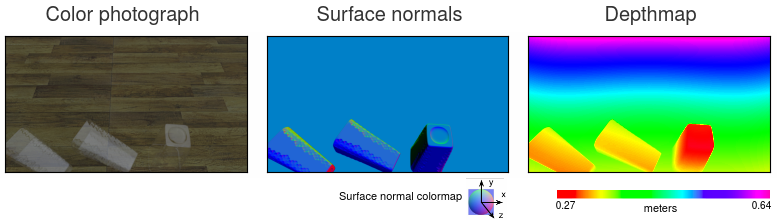
\includegraphics[width=\linewidth]{figures/Cleargrasp_data/cleargrasp_sample.png}
    \caption{Transparent objects are difficult to delineate in the color photograph since their surfaces are not distinctly visible. Furthermore, estimating depth precisely from merely one monocular color photo is a challenging problem by itself. However, given explicitly the information on the surfaces in the scene, estimation of depth of transparent objects becomes much more approachable.}
    \label{fig:cleargrasp_sample}
\end{figure}{}

We argue that this depth estimation task can simulate up to a certain extent the challenges of the HX4-PET prediction task. Following is an analysis of the involved modalities and the analogy between the two translation tasks:
 
\begin{enumerate}
    
    \item Color photograph: This modality captures the optical properties of a scene including the shades of colors on various objects and the shadows and reflections cast by the objects. Using these features, one can differentiate one object from the other and can perceive their 3D structure. However, transparent objects are difficult to delineate when relying solely on optical information due to the refractive property of their surfaces. The role of a photograph in this depth estimation task can be viewed as being analogous to the role of pCT in hypoxia map prediction problem, since both the modalities supply rich structural information regarding the overall scene but fail to be informative about one specific region -- transparent objects' structure in case of photograph image and tumor biology in case of pCT.
    
    \item Surface normals: Surface normal images encode information about 3D surface angles into a 2D image via a colormap. In the ClearGrasp dataset, surface normal renderings explicitly supply precise surface data, even for transparent objects. Therefore, this modality provides an additional layer of information that complements photographic images. Surface normals, however, fail to differentiate between parallel surfaces even when the surfaces are at different depths from the observer. In contrast, a photograph can be useful in such a situation depending on the lighting conditions. Both modalities are, therefore, mutually complementary. Surface normal image is then analogous to FDG-PET in the sense that both are informative about certain regions in the scene which their respective structural image modalities (color photograph and pCT) fail to capture, although each of them on their own is not sufficient for their respective task. 
    
    \item Depthmap: Depthmaps are single-channel 2D images whose pixel intensities represent the distance of the scene elements from the camera and are the target image modality in the simulated problem task. It has a mathematical relationship with surface normals since both are ``quantitative" images whose intensities represent some physical property. In fact, the latter can be computed from the former directly using gradients of the depth values \footnote{Algorithm for computing surface normals from depthmap: \url{https://bit.ly/3mQS588.}}. For our purpose, the depthmap serves an analogous role to HX4-PET in that tumor hypoxia is closely related to metabolism, a relationship that is physiological in nature.
    
\end{enumerate}

Using the equivalent 2D architecture of their 3D generator and discriminator networks, we apply the same three GAN systems -- Pix2Pix, CycleGAN-naive, and CycleGAN-balanced -- on this simulated problem task to obtain a prior estimation of their relative performance. In CycleGAN-balanced training, to serve a role that is analogous to ldCT-unreg in the HX4-PET synthesis task, photographic images corrupted with added Gaussian noise are used as the structural context images for their corresponding depthmaps.

A small-scale dataset for this simulated task is curated as a subset of the larger ClearGrasp set. Out of the five types of transparent objects whose images the original dataset contains, we limit our data to one object type which has a relatively simple structure -- the ``square plastic bottle". From the dataset, we select 25,000 training samples and 100 validation samples corresponding to this object to compose the subset. Each sample consists of a color photograph, a surface normal image, and a depthmap.
\chapter{Experiments}
\label{Experiments}
In experiments \ref{Expt_1} and \ref{Expt_2}, we consider Pix2Pix as an ``upperbound" image translation method, and measure the degree to which the performances of CycleGAN-naive and CycleGAN-balanced approach this upperbound. Pix2Pix is expected to perform better due to its supervised training. We used the Python package \textit{ganslate} \cite{ibrahim_hadzic_2021_5494572}, our \textit{PyTorch}-based GAN framework for image-to-image translation, to build the complete pipelines for these experiments. In conjunction with this, we used the \textit{Weights and Biases} (\textit{WandB}) online experiment tracking tool \cite{wandb} to record the training losses, validation metrics, and intermediate outputs. Additional project-specific code, including scripts, utility code, and Jupyter notebooks with step-by-step documentation for dataset preparation and image evaluation, is available in this \footnote{\url{https://github.com/Maastro-CDS-Imaging-Group/HX4-PET-translation}} public repository.



%%%%%%%%%%%%%%%%%%%%%%%%%%%%%%%%%%%%%%%%%%%%%%%%%%%%%%%%%%%%%%%%%%%%%%%%%%%%%%%%%%%%%%%%%%%%%%%%%%%%%%%%%%%%%%%%%%%%%%%%%%%%%%%%%%%%%%%%%%%%%%%
\section{Experiment 1: Testing the GANs on Depth Estimation Problem}
\label{Expt_1}

This experiment concerns with testing the GAN systems on the simulated problem of depth estimation from multimodal input comprising of photographic and surface normal images.


% ---------------------------
\subsection{Experiment Setup}

\subsubsection{Training configuration}
The curated dataset for the depth estimation task is a subset of the original ClearGrasp dataset (see \ref{ClearGrasp_Depth_Estimation}). During training, images of all three modalities are first rescaled to size 512$\times$256 and normalized to [-1, 1] range.  In Pix2Pix, $\lambda_{elem}$ value of 100 was observed to produce good results, and $\lambda_{elem}$ value of 10 is used in both CycleGANs. Similar to the optimizer configuration used in the original Pix2Pix and CycleGAN papers \cite{isola2017image, zhu2017unpaired}, we use Adam optimizer with moment parameter settings $\beta_1$=0.5 and $\beta_2$=0.999. An initial learning rate of 0.0002 is used for the generators and 0.0001 for the discriminators. We train each model with a batch size of 1 on full images for 50 epochs. The learning rates are fixed for the first 25 epochs and then linearly decayed to 0 over the next 25 epochs. Model validation is performed after each epoch. The training was run on an NVIDIA Tesla P100 SXM2 (16 GB) GPU hardware provided as part of the RWTH Compute Cluster \footnote{RWTH Compute Cluster documentation: \url{https://help.itc.rwth-aachen.de/service/rhr4fjjutttf/}}, and the training time for Pix2Pix, CycleGAN-naive, and CycleGAN-balanced models was approximately 2 hours, 4 hours, and 5 hours respectively.

\subsubsection{Evaluation settings}
We use pixel-wise mean-squared error (MSE) between the synthetic and ground truth depthmaps as the evaluation metric. Before computing the MSE, the image intensities are converted back to their original depth representation in meters.


% -------------------------------
\subsection{Result and Analysis}
Table \ref{tab:cleargrasp_quant} reports the MSE values for each model's predictions on the validation set. Pix2Pix performs the best by a large margin and is also the most robust among the three, as expected, setting the performance upperbound among the three models. CycleGAN-balanced achieves better results as compared to CycleGAN-naive. 

\begin{table}[h!]
    \small
    \centering
    \begin{tabular}{ccccccc}
        \hline
        \textbf{Method} & \textbf{MSE} \\
        \hline
        Pix2Pix    & \textbf{0.004} $\pm$ 0.005 \\
        CycleGAN-naive    & 0.192 $\pm$ 0.253 \\
        CycleGAN-balanced    & \textit{0.147} $\pm$ 0.170 \\
        \hline
    \end{tabular}
    \caption{Mean-squared error (expressed in meters$^2$) over the validation subset.}
    \label{tab:cleargrasp_quant}
\end{table}

\begin{figure}[h!]
    \centering
    \makebox[\textwidth][c]
    {   
        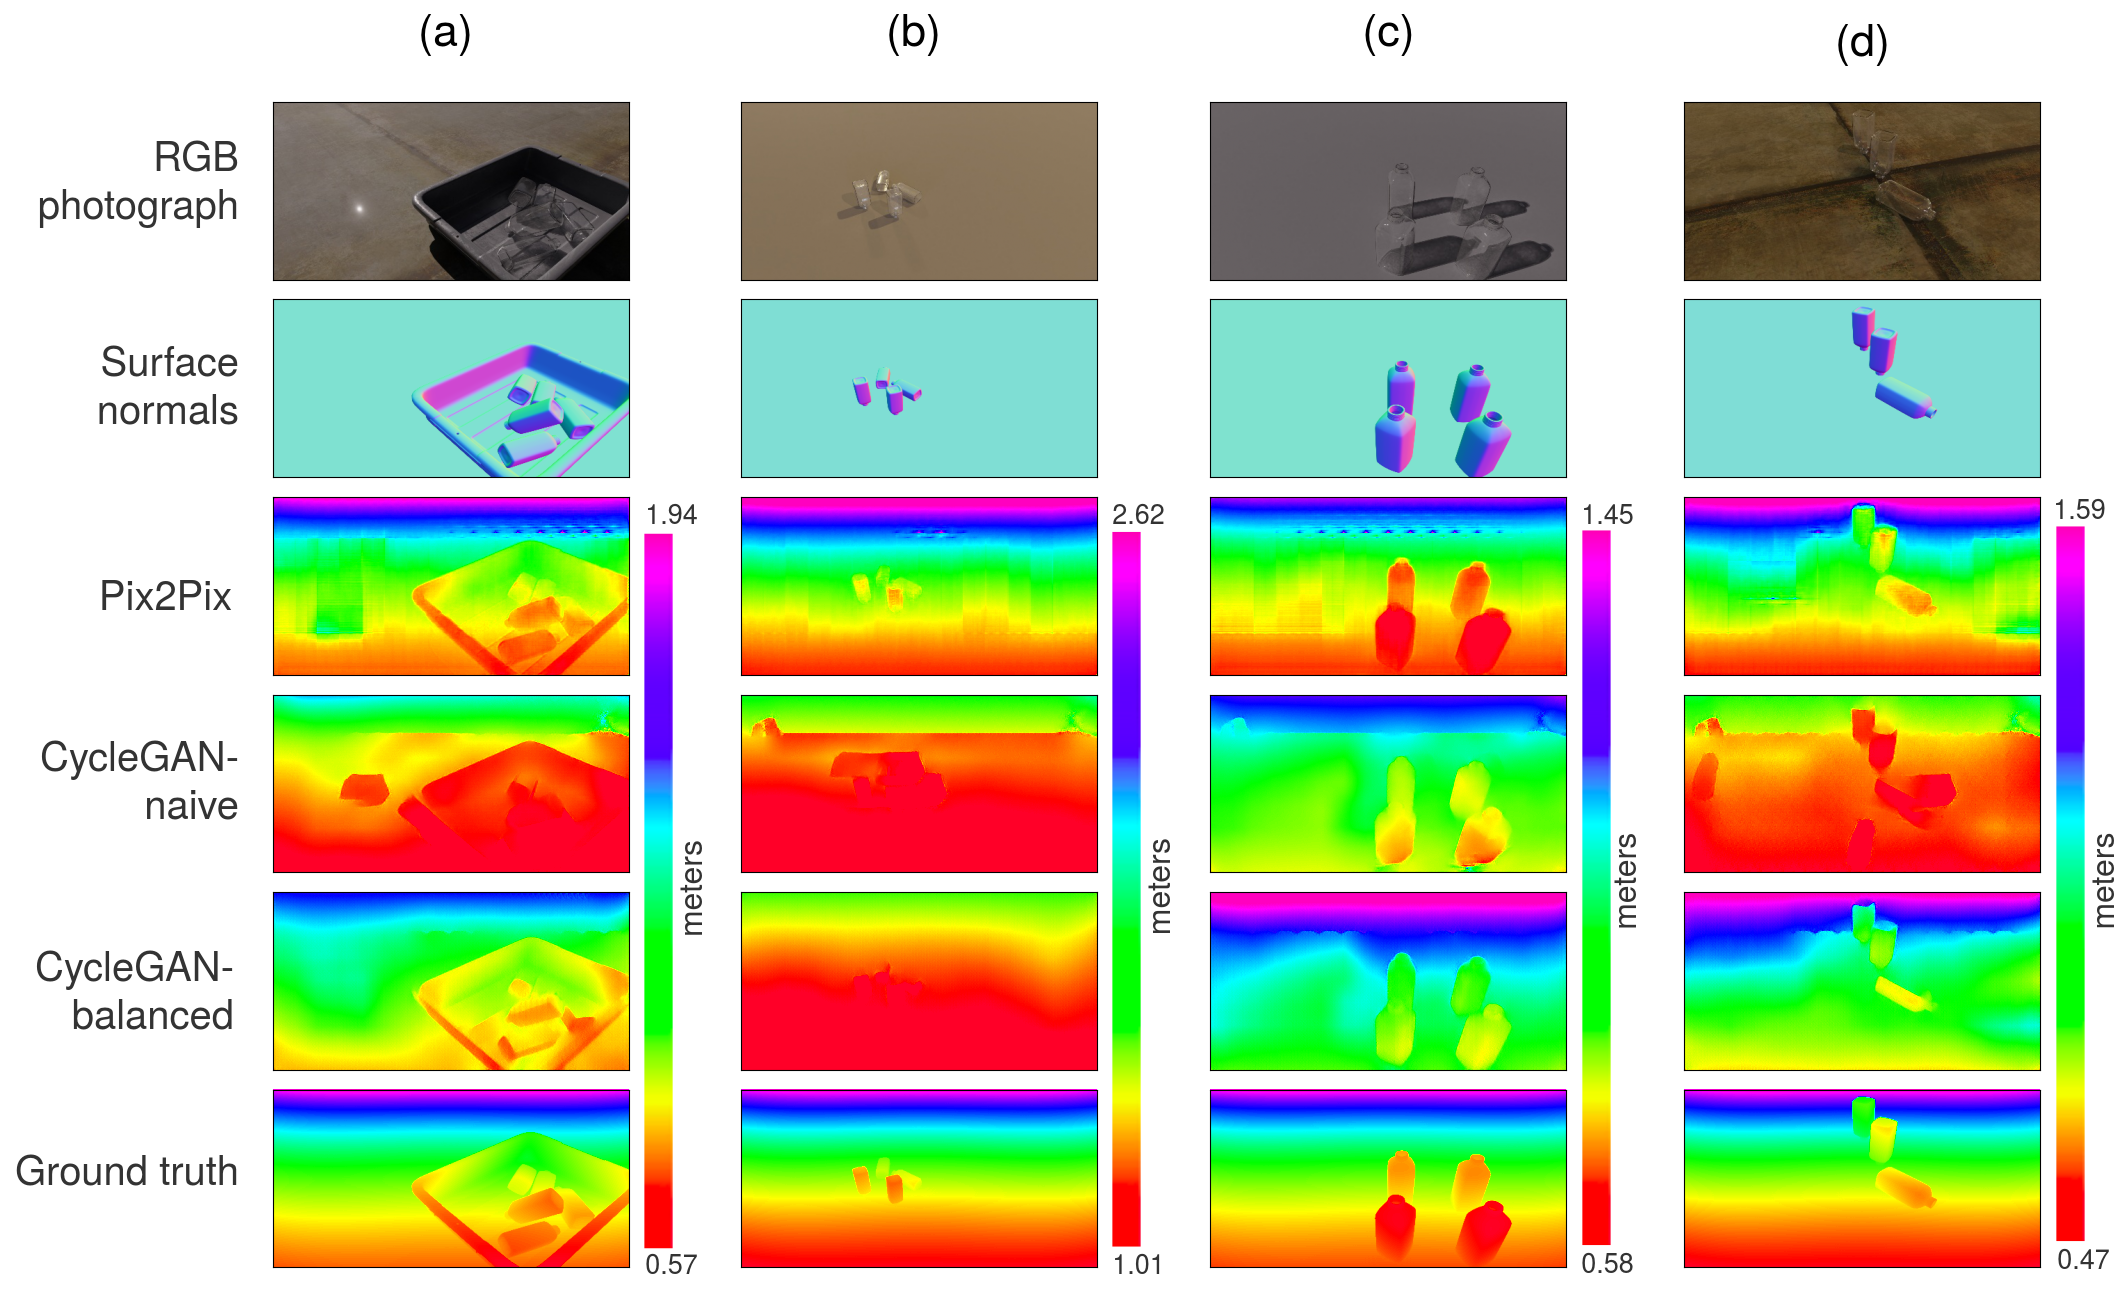
\includegraphics[width=1.05\linewidth]{figures/Expt_1/Cleargrasp_Results-viz.png}
    }
    \caption{Selected validation samples chosen to highlight the challenges in input data –- (a) a nearby tray containing transparent objects and a reflection on the floor, (b) distant objects, (c) objects casting strong shadows, and (d) a distinct cross-shaped pattern on the floor. Pix2Pix model estimated the depth of the transparent objects, other objects and the floor very close to the ground truth. CycleGAN-naive produced depthmaps with heavy artifacts, which were absent in case of CycleGAN-balanced, notably in (a) and (d).}
    \label{fig:cleargrasp_qual}
\end{figure}

Figure \ref{fig:cleargrasp_qual} shows qualitative results with samples that are representative of the MSE measurements. In general, Pix2Pix predicts the depthmaps accurately with minimal artifacts. The predictions of CycleGAN-naive contain heavy artifacts, including horizontal edges that are observed recurring across multiple images at the same position (a sign of mode collapse) and hallucinated spurious objects. The model doesn't learn the concept of depth. In case of CycleGAN-balanced, the predicted depthmaps contain a greatly reduced amount of artifacts. The model appears to have learned to infer depth, although only in a limited manner -- the depth of larger non-transparent objects (such as the tray) is estimated better compared to that of the transparent objects.

\begin{figure}[h!]
    \centering
    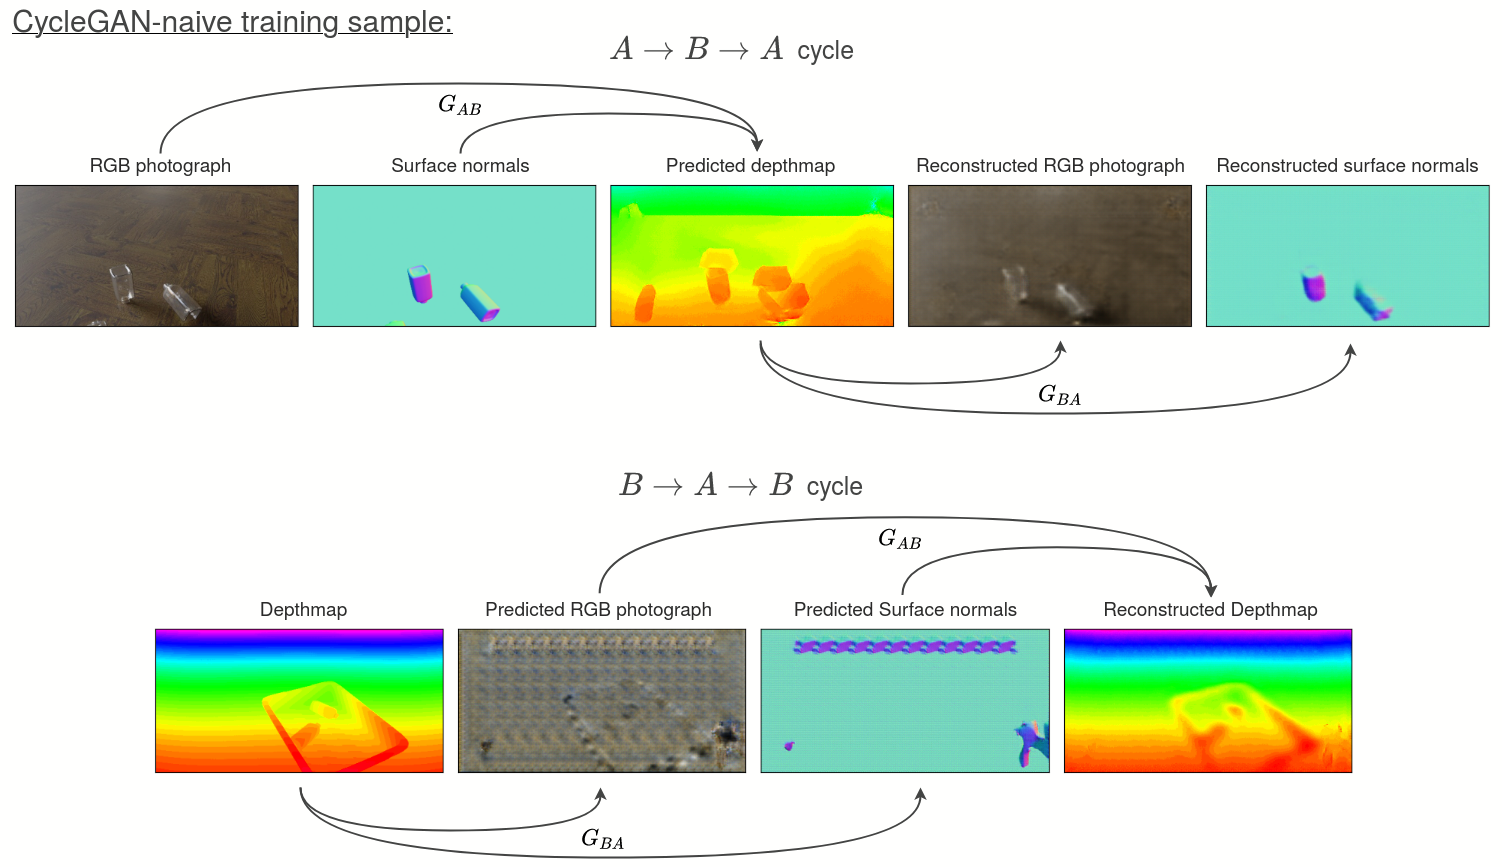
\includegraphics[width=\linewidth]{figures/Expt_1/cyclegan_naive_cycles.png}
    \caption{Single unpaired training sample and generator outputs of the fully-trained CycleGAN-naive model. In \textit{A}$\rightarrow$\textit{B}$\rightarrow$\textit{A} cycle, $G_{AB}$ predicted depthmap with hallucinated structures and yet $G_{BA}$ was able to recover back the photograph and surface normals from it. Similarly, in the \textit{B}$\rightarrow$\textit{A}$\rightarrow$\textit{B} cycle, the same $G_{BA}$ failed to compute the ``correct" photograph and surface normals from a real depthmap, and yet despite the noisy images it produced, $G_{AB}$ somehow reconstructed the depthmap from them. Here, the training problem is ill-posed and cycle-consistency fails as a result.}
    \label{fig:cleargrasp_cyclegan_naive_cycles}
\end{figure}

\begin{figure}[h!]
    \centering
    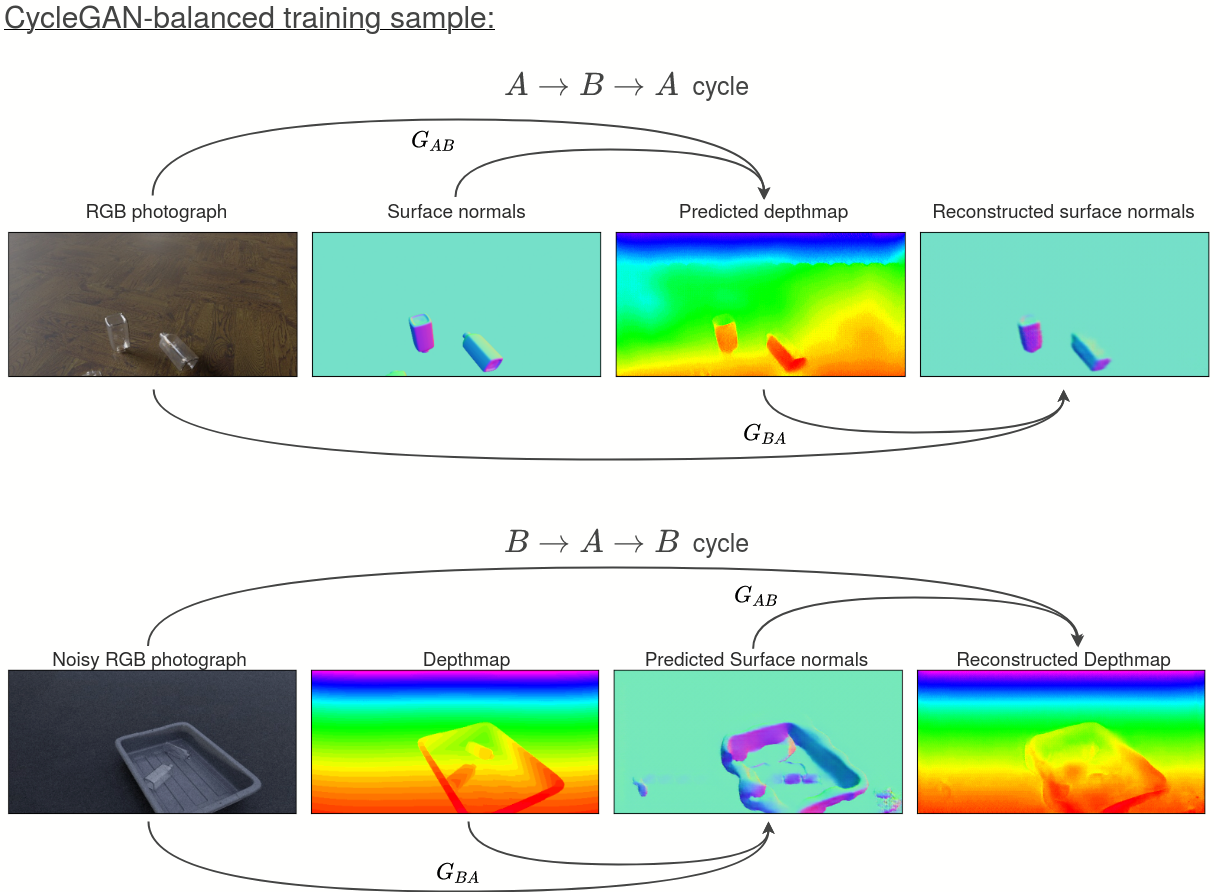
\includegraphics[width=0.8\linewidth]{figures/Expt_1/cyclegan_balanced_cycles.png}
    \caption{Single unpaired training sample and generator outputs of the fully-trained CycleGAN-balanced model. In both cycles, the translation task is mainly across surface normals and depthmaps, while the available photograph serves as a common contextual information for prediction and reconstruction. In \t cycle, the predicted surface normal image has a deformed structure. However, the reconstructed depthmap reflects this distortion and thus the cycle-consistency constraint can act on correcting it. Here, the training problem is well defined and solvable.}
    \label{fig:cleargrasp_cyclegan_balanced_cycles}
\end{figure}

To give a concrete example of the conceptual issues with CycleGAN-naive (described earlier in \ref{cyclegan}), the outputs produced by both its generators are visualized and compared with the generator outputs of CycleGAN-balanced. Figures \ref{fig:cleargrasp_cyclegan_naive_cycles} and \ref{fig:cleargrasp_cyclegan_balanced_cycles} show the outputs of the fully-trained CycleGAN-naive and CycleGAN-balanced models, respectively, given an equivalent set of unpaired input images. In Figure \ref{fig:cleargrasp_cyclegan_naive_cycles}, the generator $G_{AB}$ of CycleGAN-naive in the \textit{A}$\rightarrow$\textit{B}$\rightarrow$\textit{A} cycle produces an incorrect depthmap containing spurious objects from the given photographic and surface normal images. $G_{BA}$ then not only uses this flawed depthmap to accurately reconstruct the objects in the original photograph and surface normal image, but also manages to perfectly recover the colors in the photograph. In order to satisfy cycle-consistency, $G_{AB}$ encodes the information about the transparent objects' shape as well as the photograph's optical information into the depthmaps, which $G_{BA}$ uses to almost completely recover the input images, especially the color photograph. The model learns to bypass the content-preservation requirement which cycle-consistency is intended to indirectly encourage. In \textit{B}$\rightarrow$\textit{A}$\rightarrow$\textit{B} cycle, the generator $G_{BA}$, which in previous cycle relied on information encoded as noise in the fake depthmap images, now fails to predict the ``correct" photograph and surface normals given a real (and noise-free) depthmap, thereby producing highly noisy images completely devoid of any meaningful features. However, $G_{AB}$ still reconstructs the depthmap from these noisy images, indicating that the $G_{BA}$ must have encoded relevant information, possibly as noise, into its output. Cycle-consistency is bypassed in this case as well. The problem arises because although the task of learning $G_{AB}$ might be solvable, learning its inverse ($G_{BA}$) isn't, since such a unique inverse mapping doesn't exist. The learning problem as formulated for the CycleGAN-naive model is ill-posed, in the sense that there is no solution to it, and therefore, the training would fail inevitably. 

On the other hand, the outputs of CycleGAN-balanced generators shown in Figure \ref{fig:cleargrasp_cyclegan_balanced_cycles} highlight the system's improved capability of learning the relevant mappings. Here, the main participant modalities of the translation task are the surface normal image and the depthmap. Neither of the generator tasks involves synthesizing the color photographs from the less information-rich modalities. Using the given photographic images always as an input component for the generators provides them shared contextual information within each cycle. The unpaired learning problem for CycleGAN-balanced is better formulated and solvable, and hence the training process can yield a suitable translation model.



%%%%%%%%%%%%%%%%%%%%%%%%%%%%%%%%%%%%%%%%%%%%%%%%%%%%%%%%%%%%%%%%%%%%%%%%%%%%%%%%%%%%%%%%%%%%%%%%%%%%%%%%%%%%%%%%%%%%%%%%%%%%%%%%%%%%%%%%%%%%%%%
\section{Experiment 2: Image Quality Metrics For Synthetic HX4-PET Assessment}
\label{Expt_2}
This experiment focuses on evaluation of the GAN systems for the HX4-PET synthesis task. Global quality of the HX4-PET-syn images is assessed using general metrics of image quality and similarity. Additionally, the applicability of these metrics in tracking model convergence during training is explored.


% ---------------------------
\subsection{Experiment Setup}

\subsubsection{Training configuration}
The dataset used in this experiment is the Maastro Lung HX4-PET dataset after undergoing the preparation steps described in \ref{Data_Processing}. The patch-based training pipeline described in \ref{training_pipeline} is used for all model training. Because a the models are trained on sets of patches extracted from the images using stochastic strategies, the notion of an ``epoch" doesn't exist here. Instead, the number of iterations is used as a measure of training duration, where an iteration is composed of sampling a set of image patches from the full images, performing the required forward passes through the networks, and updating the weights of all the networks in the GAN system. We train each GAN model for 60,000 iterations. The scaling factor $\lambda_{elem}$ for the element-wise loss in Pix2Pix is set to 10, and a $\lambda_{cyc}$ of 10 is used for the cycle-consistency loss in the CycleGANs. Similar to experiment \ref{Expt_1}, Adam optimizer is used with settings $\beta_1$=0.5 and $\beta_2$=0.999. Initial learning rates 0.0002 for the generators and 0.0001 for the discriminators are used during the first 30,000 iterations followed by linearly decaying the learning rate values to 0 over the remaining 30,000 iterations. Model validation is performed every 1000 iterations. All models are trained with batch size 1.

Training was performed on an NVIDIA Tesla V100 SXM2 (32 GB) GPU provided by Data Science Research Infrastructure (DSRI) \footnote{DSRI documentation: \url{https://maastrichtu-ids.github.io/dsri-documentation/}} of Maastricht University. The 3D training of the Pix2Pix, CycleGAN-naive, and CycleGAN-balanced models took 9.5 hours, 13 hours, and 15.25 hours, respectively. 


\subsubsection{Evaluation settings}
The set of six image quality and similarity metrics described in \ref{image_quality_metrics} are used to assess the quality of HX4-PET-syn images, given the corresponding ground truth HX4-PET-reg images. The intensity scale is divided into 100 bins while computing NMI (for entropy calculation) and global histogram distance.

Additionally, a systematic visual inspection of the synthetic images is performed to identify failure modes that are typical to each GAN model. This would also enable validating the assessment of the image quality metrics. For each patient in the validation set, each model's predicted HX4-PET-syn images were visualized and inspected along all three axes -- axial, sagittal and coronal -- using the \textit{3D Slicer} visualization software \cite{kikinis20143d} under a window of [0, 1.3] SUV. This window is chosen so that the most of the variation in image intensities could be covered. The following set of image degradation criteria are defined to guide the visual inspection:

\begin{enumerate}
    \item \textit{Presence of background noise patterns:} It is well known that checkerboard artifacts can occur in GAN generated images usually due to the the nature of the transposed convolution operation used in upsampling layers \cite{odena2016deconvolution}. This criterion aims at judging the images based on the presence of such periodic noise patterns in the region outside the body where the hypoxia signal is supposed to be zero. This criterion would be satisfied only when severe amount of noise is present such that it is readily visible to the observer in most slices along all three axes of the 3D image.
    
    \item \textit{Presence of noise patterns in the body region:} Checkerboard and other periodic noise patterns in the background may be absent in better performing models because all models were trained on body-masked images whose background intensities were set to zero signal value (0 SUV in PET and -1024 HU (air) in CT). Regardless, such noise can also possibly occur \textit{within} the body region, i.e. the foreground of the image. This criterion aims to account for this, and to satisfy it the noise must be severe enough to be easily detectable by the observer, must be wide spread in roughly the central parts of the body area (i.e. away from boundary regions) and recurring across multiple slices along all three image axes. 
    
    \item \textit{Presence of hallucinated structures:} Generated scans can possibly contain structures which wouldn't be characteristic of human physiology, which might have been constructed by the model to increase the resemblance of the image to the target distribution samples. Many of such structures could be conspicuous enough to be noticeable to non-experts, however others would be too challenging even for trained professionals to discover. This is because unlike CT which shows anatomical structure in high detail, PET images, and especially HX4-PET, show only vague and diffused forms. The synthetic HX4-PET is bound to have at least some differences in these forms as compared to the ground truth, and therefore it is difficult to draw a line past which the differences can be deemed a hallucinated object. Hence, this criterion focuses on the former, more conspicuous, type of artificial structures. For example, isolated high-intensity objects with globular or ring-like shape, similar to common tumor hypoxia signatures, in regions where they shouldn't exist. Using the ground truth as reference, detection of even a single such structure in a predicted image would satisfy this criterion.
    
    \item \textit{Breaks in the existing structure:} Abrupt breaks in structure, for example, holes and gaps with sharp edges, inside the patient's body region in the generated images can occur when the model has not learned relevant anatomical features. Many such glitches can be easily detected by an untrained observer, and this criterion aims to account for their presence in the synthetic HX4-PET images. One or more severe gaps of such type in the image foreground would satisfy this criterion.
\end{enumerate}



% ------------------------------------------------------------------
\subsection{Result and Analysis 1: Evaluating Fully Trained Models}
Performance of the three 3D models as measured by the six image metrics is reported in Table \ref{tab:hx4_image_quality_quant}. Pix2Pix emerges to be the best performing model as evaluated by all six metrics, followed by CycleGAN-balanced whose performance values are very close to those of Pix2Pix. CycleGAN-naive performs the worst, as agreed by all the metrics. Borda counting based on the individual performance rankings of the metrics resulted in the same global ranking on the models -- Pix2Pix as the best model, followed by CycleGAN-balanced and finally CycleGAN-naive.

% % Original table
% \begin{table}[h!]
%     \scriptsize
%     \centering
%     \makebox[\textwidth][c]
%     {
%         \begin{tabular}{ccccccc}
%             \textbf{Method}   & \textbf{MSE}   & \textbf{MAE}   & \textbf{PSNR}   & \textbf{SSIM}   & \textbf{NMI}   & \textbf{Histogram dist.} \\
%             \hline
%             Pix2Pix   & \textbf{0.009} $\pm$ 0.006   & \textbf{0.049} $\pm$ 0.008   & \textbf{27.467} $\pm$ 1.946   & \textbf{0.582} $\pm$ 0.086   & \textbf{1.215} $\pm$ 0.016   & \textbf{0.563} $\pm$ 0.160 \\
%             CycleGAN-naive   & 0.043 $\pm$ 0.004   & 0.185 $\pm$ 0.006   & 20.217 $\pm$ 2.032   & 0.190 $\pm$ 0.044   & 1.099 $\pm$ 0.009   & 1.289 $\pm$ 0.201 \\
%             CycleGAN-balanced   & \textit{0.016} $\pm$ 0.008   & \textit{0.067} $\pm$ 0.010   & \textit{25.119} $\pm$ 1.812   & \textit{0.5} $\pm$ 0.075   & \textit{1.181} $\pm$ 0.015   & \textit{0.662} $\pm$ 0.124 \\
%         \end{tabular}
%     }
%     \caption{Performance on the Maastro Lung HX4-PET validation set. Best and second-to-best values are highlighted with bold and italics font, respectively. Performance of the unpaired CycleGAN-balanced model reaches close to that of the paired Pix2Pix model.}
%     \label{tab:hx4_image_quality_quant}
% \end{table}

% Transposed table
\begin{table}[h!]
    \footnotesize
    \centering
    \begin{tabular}{l || lll}
         \hline
         \textbf{Method} $\rightarrow$  & Pix2Pix                      & CycleGAN-naive      & CycleGAN-balanced            \\
         \hline
         \textbf{MSE}                   & \textbf{0.009} $\pm$ 0.006   & 0.043 $\pm$ 0.004   & \textit{0.016} $\pm$ 0.008   \\
         \textbf{MAE}                   & \textbf{0.049} $\pm$ 0.008   & 0.185 $\pm$ 0.006   & \textit{0.067} $\pm$ 0.010   \\
         \textbf{PSNR}                  & \textbf{27.467} $\pm$ 1.946  & 20.217 $\pm$ 2.032  & \textit{25.119} $\pm$ 1.812  \\
         \textbf{SSIM}                  & \textbf{0.582} $\pm$ 0.086   & 0.190 $\pm$ 0.044   & \textit{0.5} $\pm$ 0.07      \\
         \textbf{NMI}                   & \textbf{1.215} $\pm$ 0.016   & 1.099 $\pm$ 0.009   & \textit{1.181} $\pm$ 0.015   \\
         \textbf{Histogram distance}    & \textbf{0.563} $\pm$ 0.160   & 1.289 $\pm$ 0.201   & \textit{0.662} $\pm$ 0.124   \\
         \hline
         \textbf{Performance ranking}   & \textbf{1}                   & 3                   & \textit{2}                   \\
         \hline        
    \end{tabular}
    \caption{Performance on the Maastro Lung HX4-PET validation set. Best and second-to-best values are highlighted with bold and italics font, respectively. Performance of the unpaired CycleGAN-balanced model reaches close to that of the paired Pix2Pix model. The final performance ranking is calculated by combining each ranking produced by metric, with Borda count.}
    \label{tab:hx4_image_quality_quant}
\end{table}

Results of the visual inspection are reported in Table \ref{tab:hx4_image_quality_inspection}. Figure \ref{fig:hx4_image_quality_inspection_viz} compares the predictions of the models for different patients and highlights failure modes typical to each model.

% % Original table
% \begin{table}[h!]
%     \footnotesize
%     \centering
%     \makebox[\textwidth][c]
%     {
%         \begin{tabular}{ccccc}
%             \textbf{Method}   & \textbf{Background noise}   & \textbf{Foreground noise}   & \textbf{Hallucinated structures}   & \textbf{Broken structures}   \\
%             \hline
%             Pix2Pix   & \textbf{0\%} (0/19)   & \textbf{26.3\%} (5/19)   & \textbf{10.5\%} (2/19)   & \textbf{57.9\%} (11/19)   \\
%             CycleGAN-naive   & 100\% (19/19)   & 100\% (19/19)   & 57.9\% (11/19)   & 100\% (19/19)   \\
%             CycleGAN-balanced   & \textit{42.1\%} (8/19)   & \textit{42.1\%} (8/19)   & \textit{31.6\%} (6/19)   & \textit{89.5\%} (17/19)   \\
%         \end{tabular}
%     }
%     \caption{Fraction of the total validation set images meeting the corresponding image degradation criteria. Best and second-to-best values are highlighted with bold and italics font, respectively.}
%     \label{tab:hx4_image_quality_inspection}
% \end{table}

% Transposed table
\begin{table}[h!]
    \footnotesize
    \centering
    \begin{tabular}{l || lll}
         \hline
         \textbf{Method} $\rightarrow$     & Pix2Pix                    & CycleGAN-naive  & CycleGAN-balanced          \\
         \hline
         \textbf{Background noise}         & \textbf{0\%} (0/19)        & 100\% (19/19)   & \textit{42.1\%} (8/19)     \\
         \textbf{Foreground noise}         & \textbf{26.3\%} (5/19)     & 100\% (19/19)   & \textit{42.1\%} (8/19)     \\
         \textbf{Hallucinated structures}  & \textbf{10.5\%} (2/19)     & 57.9\% (11/19)   & \textit{31.6\%} (6/19)     \\
         \textbf{Broken structures}        & \textbf{57.9\%} (11/19)    & 100\% (19/19)   & \textit{89.5\%} (17/19)    \\
         \hline
    \end{tabular}
    \caption{Fraction of the total validation set images meeting the corresponding image degradation criteria. Best and second-to-best values are highlighted with bold and italics font, respectively.}
    \label{tab:hx4_image_quality_inspection}
\end{table}


\begin{figure}
    \centering
    \makebox[\textwidth][c]
    {
        \includegraphics[width=1.4\linewidth]{figures/Expt_2/image_quality/image_quality_inspection_viz-2.png}
    }
    \caption{Corresponding slices of the inputs, the ground truth and the predictions. All PET images are overlaid on the corresponding pCT. Gross tumor volumes (GTV) are delineated with green contours. Severe background noise is visible in CycleGAN-naive outputs, which also penetrates into the foreground as seen in (a). Sharp edged holes in (a) and a rift in (b) (cyan ellipses), a common occurrence in CycleGAN-naive predictions. In (d), the Pix2Pix output shows structure break at the bottom likely caused due to model being trained on faulty ground truth (cyan bounding boxes). In (c), the outputs of CycleGAN-naive and CycleGAN-balanced have a hallucinated ring-shaped hypoxia signature near the heart (cyan arrows).}
    \label{fig:hx4_image_quality_inspection_viz}
\end{figure}

None of Pix2Pix predictions contained severe background noise patterns, as opposed to the predicted images from CycleGAN-naive, all of which were severely corrupted by noise in both background and foreground. CycleGAN-balanced stands almost half-way between the other two models in terms of background and foreground noise, although none of its outputs contained noise as severe as in case of CycleGAN-naive. The background noise is easily visible in Figure \ref{fig:hx4_image_quality_inspection_viz}a. The presence of greater noise in CycleGAN-naive is likely to be related to its conceptual problem related to non-invertibility. The \textit{A}$\rightarrow$\textit{B} translation involves predicting hypoxia map from pCT and FDG-PET, which can have a unique solution. Whereas its reverse, the \textit{B}$\rightarrow$\textit{A} translation, involves computing ideally exact pCT and FDG-PET given only the hypoxia map information, which is not possible unless the model encodes the extra information, as noise or artifacts, in the hypoxia image.

Structural breaks and holes were observed in a majority of all models' outputs. These were, however, more severe and numerous in case of CycleGAN-naive and CycleGAN-balanced, more in the former than in the latter. Pix2Pix had comparably lower number of these faults. A notable difference is that while many of such structural faults appeared in roughly the middle and upper regions of the body in predicted images in case of the two CycleGANs, most of them in Pix2Pix predictions were located in the bottom-most axial slices. These are shown in Figures \ref{fig:hx4_image_quality_inspection_viz}a, \ref{fig:hx4_image_quality_inspection_viz}b and \ref{fig:hx4_image_quality_inspection_viz}d. A likely cause of this is the registration imperfections in the ground truth HX4-PET-reg images, many of which had missing signal in parts of the bottom axial slices. Pix2Pix training, which assumes voxel-to-voxel similarity across input and output images, might have been affected by this training noise resulting in a model that couldn't accurately predict the hypoxia patterns in the bottom slices. On the other hand, the CycleGAN models which were trained on unpaired and unregistered HX4-PET-unreg images did not exhibit structural breaks of this kind, and in fact, during validation, were able to predict plausible hypoxia patterns in the bottom slices of their predictions whose corresponding ground truths themselves were faulty. This is visible in Figure \ref{fig:hx4_image_quality_inspection_viz}d. The fact that the validation set's ground truth HX4-PET-reg images have this issue of missing signal may create another problem -- if the reference image itself is partly incomplete in some region and if a model predicts a plausible hypoxia signal in that region of its predicted image, evaluating the image quality, especially using the voxel-wise difference metrics, can result in an incorrect assessment. However, this may not pose a serious issue here because first, only a small portion of the signal in entire ground truth image is missing, and second, the models being compared have significant differences in performance as the visual inspection revealed.

Finally, the type of image degradation related to the presence of hallucinated structures was observed more commonly in case of CycleGAN-naive and CycleGAN-balanced as compared to Pix2Pix. This was mainly characterized by the insertion of ring-shaped hypoxia signatures in regions near the heart and the upper abdomen. However, such signatures are a common feature only within the tumor where parts of its periphery are actually hypoxic. A likely reason of this pattern to occur in other regions in the predictions of the two CycleGANs is the failure to learn relevant anatomical features from the pCT and depending more heavily on features related to metabolic activity from FDG-PET in these regions. The Pix2Pix model trained directly in a supervised manner mostly managed to avoid this issue. This can be seen in Figure \ref{fig:hx4_image_quality_inspection_viz}c.

In summary, the results of the visual inspection reflect the quantitative evaluation results. Pix2Pix produced synthetic HX4-PET images that are visually highly similar to the ground truth, mostly owing to its supervised training. However, because it was trained in the supervised manner on imperfect ground truth images, it also produced locally specific structure breaks in its predictions. Among the unpaired GAN systems, CycleGAN-balanced showed great improvement over CycleGAN-naive and was able to greatly reduce degradation caused by noise and hallucinated structures.


% ------------------------------------------------------------------------------
\subsection{Result and Analysis 2: Analyzing Model Convergence during Training}
\label{cycelgan_convergence}


\subsubsection{Adversarial training of CycleGAN} 
Informally, model convergence refers to a case where the machine learning model's loss approaches a certain optimal value with a decreasing rate over the training iterations. In GAN training, two networks are simultaneously optimized with conflicting objectives. In theory, a Vanilla GAN model asymptotically converges to an equilibrium state where the generator perfectly models the data distribution and the discriminator's prediction over real and fake data is 0.5 on average, i.e. it can only do random guessing \cite{goodfellow2014generative}. This stands, of course, only under the condition that the discriminator is trained to optimality for each iteration of the generator's update. In practice, the discriminator is updated just once per generator update, but since the discriminator's task of binary classification is simpler than the generator's task of image synthesis, the discriminator is likely to learn faster and remain competitive with the generator in the corresponding iterations. In this part of the experiment, GAN convergence is analyzed empirically for the CycleGAN-naive and CycleGAN-balanced systems, by reasoning based on their recorded training losses.

The least-squares adversarial loss used in our CycleGAN models is shown in Equation \ref{eq:gan_loss}.
\begin{equation}
    \begin{aligned}
    L(G) &= E_{x \sim p_{data}(x)} [(1 - D(G(x)))^2] \\
    L(D) &= E_{x \sim p_{data}(x)} [D(G(x))^2] + E_{y \sim p_{data}(y)} [(1 - D(y))^2] 
    \end{aligned}
    \label{eq:gan_loss}
\end{equation}
where $G$ and $D$ represent a generator ($G_{AB}$ or $G_{BA}$) and the corresponding discriminator ($D_B$ or $D_A$), respectively. $x$ represents an image from the input domain of the generator $G$, and $y$ represents an image from its target domain. This general representation is used here for simplicity. 

During training, $G$ and $D$ are updated in an alternating manner. As the training progresses and if the training is stable, both $G$ and $D$ improve at a similar rate maintaining a competitive behavior. Depending on the extent of the stability, losses of both models either stay constant reaching an equilibrium or oscillate around the equilibrium values. Such an equilibrium state is reached when, after every update, $G$'s output images are good enough to force $D$ into random guessing and predicting a validity value of 0.5 on average for both real and fake images. Then according to Equation \ref{eq:gan_loss}, the equilibrium state loss values $L(G^*)$ and $L(D^*)$ are 0.25 and 0.5, respectively. 

\begin{figure}[h!]
    \begin{subfigure}{.5\textwidth}
        \centering
        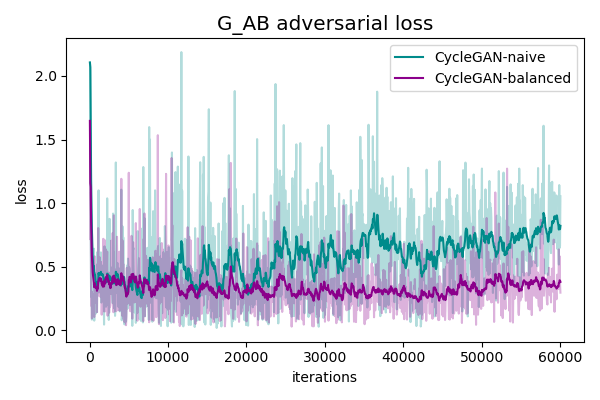
\includegraphics[width=.95\linewidth]{figures/Expt_2/gan_convergence/loss_G_AB.png}
        \caption{}
        \label{fig:loss_G_AB}
    \end{subfigure}
    \begin{subfigure}{.5\textwidth}
        \centering
        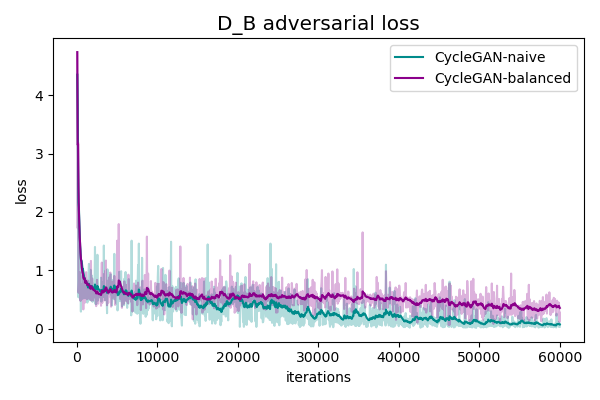
\includegraphics[width=.95\linewidth]{figures/Expt_2/gan_convergence/loss_D_B.png}
        \caption{}
        \label{fig:loss_D_B}
    \end{subfigure}
    \newline

    \begin{subfigure}{.5\textwidth}
        \centering
        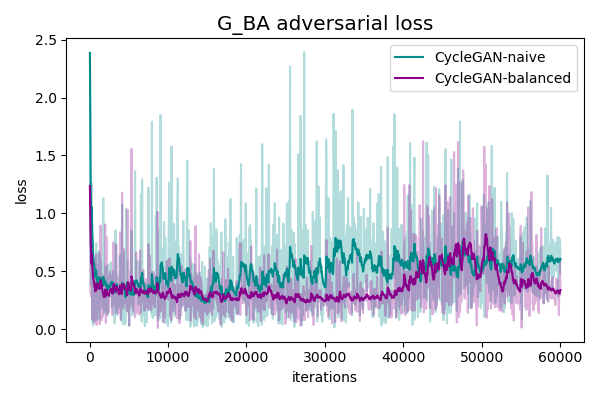
\includegraphics[width=.95\linewidth]{figures/Expt_2/gan_convergence/loss_G_BA.png}
        \caption{}
        \label{fig:loss_G_BA}
    \end{subfigure}
    \begin{subfigure}{.5\textwidth}
        \centering
        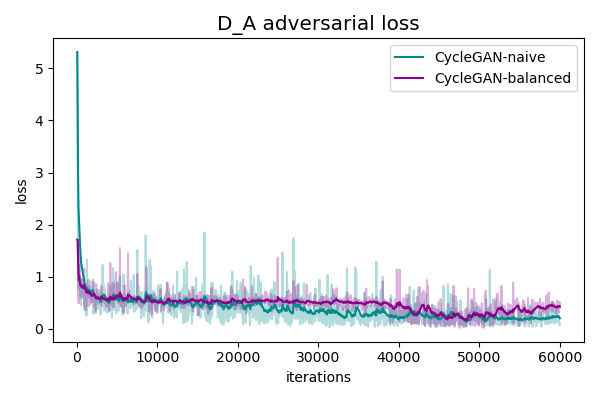
\includegraphics[width=.95\linewidth]{figures/Expt_2/gan_convergence/loss_D_A.png}
        \caption{}
        \label{fig:loss_D_A}
    \end{subfigure}
    
    \begin{subfigure}{.5\textwidth}
        \centering
        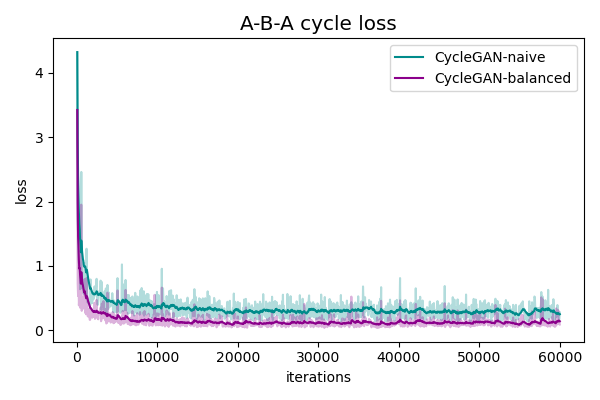
\includegraphics[width=.95\linewidth]{figures/Expt_2/gan_convergence/loss_cycle_A.png}
        \caption{}
        \label{fig:loss_cycle_A}
    \end{subfigure}
    \begin{subfigure}{.5\textwidth}
        \centering
        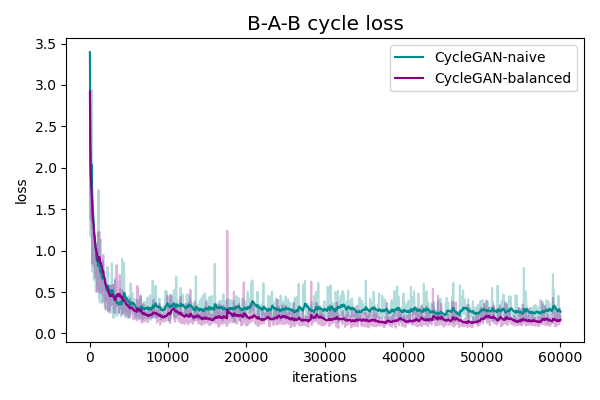
\includegraphics[width=.95\linewidth]{figures/Expt_2/gan_convergence/loss_cycle_B.png}
        \caption{}
        \label{fig:loss_cycle_B}
    \end{subfigure}

    \caption{Adversarial and cycle consistency loss curves for the two CycleGAN models. Exponential moving average smoothing was applied to each to show the general trend.}
    \label{fig:cyclegan_losses}
\end{figure}{}

Figure \ref{fig:cyclegan_losses} shows the adversarial training loss plots for CycleGAN-naive and CycleGAN-balanced. The aforementioned general reasoning is now applied independently to the two generator-discriminator pairs of the CycleGAN system. Consider the \textit{A}$\rightarrow$\textit{B} direction first. The adversarial loss $L({G_{AB})}$ of CycleGAN-balanced was closer to the equilibrium value than the that of CycleGAN-naive was, whose $G_{AB}$ was much more unstable and diverged away more significantly from around 25,000$^{th}$ iteration. This effect relates to the corresponding discriminator $D_B$ of CycleGAN-naive starting to overpower its $G_{AB}$ at around the same period. Discriminator $D_B$ of CycleGAN-balanced was maintained more stably around its equilibrium loss value of 0.5 over the full training period. Now looking at the \textit{B}$\rightarrow$\textit{A} direction, a similar pattern is observed. Except here, the generator-discriminator pair $G_{BA}$ and $D_A$ of CycleGAN-balanced appeared to destabilize and deviate away between 40,000$^{th}$ and 50,000$^{th}$ iteration, although eventually regaining stability near the end of the training. 

Additionally, cycle-consistency in CycleGAN-balanced was maintained to a greater extent almost throughout the training period as compared to CycleGAN-naive. The desirable training characteristics shown by the CycleGAN-balanced system can be attributed to its design modification.

\begin{figure}[h!]
    \makebox[\textwidth][c]
    {
        \begin{subfigure}{.4\textwidth}
            \centering
            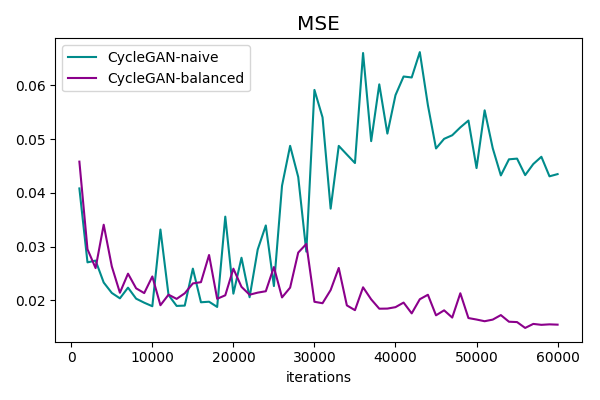
\includegraphics[width=\linewidth]{figures/Expt_2/gan_convergence/metric_val_mse.png}
            \caption{}
            \label{fig:metric_val_mse}
        \end{subfigure}
        \begin{subfigure}{.4\textwidth}
            \centering
            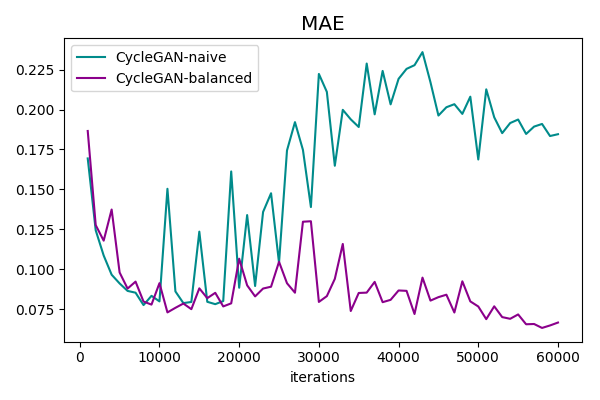
\includegraphics[width=\linewidth]{figures/Expt_2/gan_convergence/metric_val_mae.png}
            \caption{}
            \label{fig:metric_val_mae}
        \end{subfigure}
        \begin{subfigure}{.4\textwidth}
            \centering
            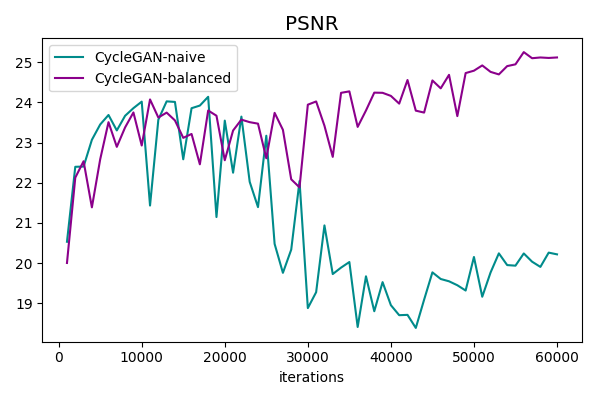
\includegraphics[width=\linewidth]{figures/Expt_2/gan_convergence/metric_val_psnr.png}
            \caption{}
            \label{fig:metric_val_psnr}
        \end{subfigure}
    }
    \newline
    \makebox[\textwidth][c]
    {
        \begin{subfigure}{.4\textwidth}
            \centering
            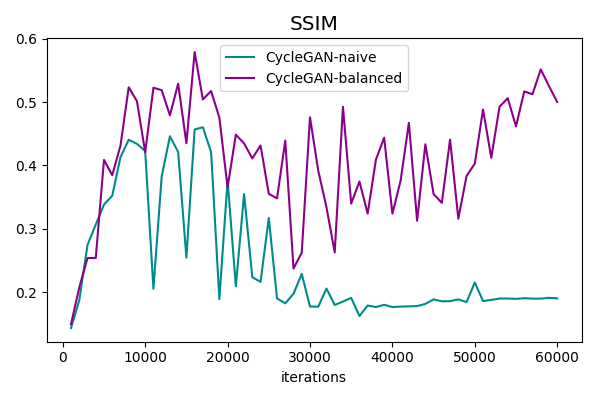
\includegraphics[width=\linewidth]{figures/Expt_2/gan_convergence/metric_val_ssim.png}
            \caption{}
            \label{fig:metric_val_ssim}
        \end{subfigure}
        \begin{subfigure}{.4\textwidth}
            \centering
            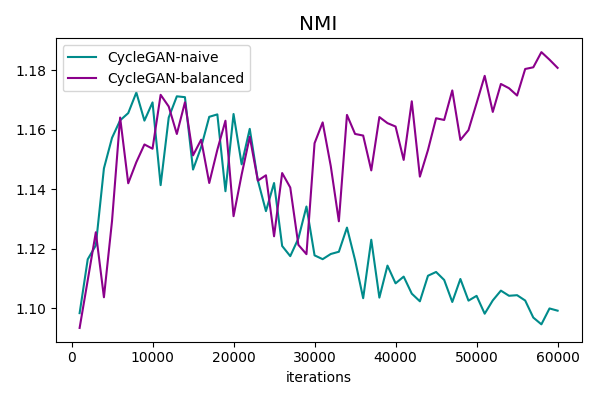
\includegraphics[width=\linewidth]{figures/Expt_2/gan_convergence/metric_val_nmi.png}
            \caption{}
            \label{fig:metric_val_nmi}
        \end{subfigure}
        \begin{subfigure}{.4\textwidth}
            \centering
            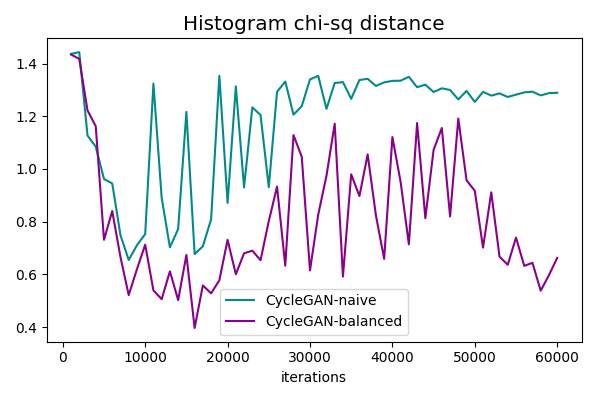
\includegraphics[width=\linewidth]{figures/Expt_2/gan_convergence/metric_val_histogram_chi2.png}
            \caption{}
            \label{fig:metric_val_histogram_chi2}
        \end{subfigure}
    }
    \caption{Validation metrics for the two CycleGAN models over the training period.}
    \label{fig:cyclegan_metrics}
\end{figure}{}

\subsubsection{Generalization performance} 
Next, we examine whether the same trend as was observed in the training convergence parameters is also reflected in the models' generalization performance on the validation set. Figure \ref{fig:cyclegan_metrics} plots the six validation metrics for the CycleGAN models over the training period. The voxel-wise difference metrics -- MSE, MAE and PSNR -- show a generally consistent improvement in CycleGAN-balanced reflecting its relatively stable training. However, the metrics based on image intensity statistics -- SSIM, NMI and histogram $\chi^2$ distance -- show a brief, yet prominent, performance dip in the model halfway into the training suggesting a temporary drop in its generalizability. CycleGAN-naive followed a generally similar trend as CycleGAN-balanced up until approximately 25,000$^{th}$ iteration -- i.e. gradual improvement in the beginning followed by a performance dip. Though, contrary to CycleGAN-balanced, it was unable to recover its generalizability and continued to deviate. This correlates with the significant instability and divergence of the CycleGAN-naive model observed in the training convergence parameters at about the same period in the training process.

In summary, the image quality metrics applied on validation data were indeed informative about model convergence. Additionally, since some of them measured different properties of the generated images, they can be helpful in effectively tracking model generalizability.



%%%%%%%%%%%%%%%%%%%%%%%%%%%%%%%%%%%%%%%%%%%%%%%%%%%%%%%%%%%%%%%%%%%%%%%%%%%%%%%%%%%%%%%%%%%%%%%%%%%%%%%%%%%%%%%%%%%%%%%%%%%%%%%%%%%%%%%%%%%%%%%
\section{Experiment 3: Application-specific Downstream Tasks}
\label{Expt_3}
This experiment focuses on clinically focused evaluation of the synthetic hypoxia PET images by quantifying hypoxia inside the gross tumor volume (GTV).


% ---------------------------
\subsection{Experiment Setup}
HX4-PET-syn images are computed for each patient in the validation set using the fully trained models, their units converted to SUV scale, and stored as NRRD files. The images are then loaded and analyzed. Each HX4-PET-syn image and its corresponding ground truth HX4-PET-reg are first cropped to a bounding box containing just the GTV. The GTV mask is then applied to the images, and intensities outside the mask are set to 0. Next, the GTV SUV values are converted to the tumor-to-background ratio (TBR) by dividing each GTV voxel's SUV with $SUV_{aorta-mean}$. From this point onward, the different hypoxia quantification metrics are computed separately as follows:

\begin{enumerate}
    
    \item \textit{MSE-GTV and SSIM-GTV:} MSE and SSIM are calculated only on the GTV voxels using array masking.
    
    \item \textit{Hypoxic tumor classification:} One of the ways of classifying the tumor as hypoxic or non-hypoxic is by calculating the total physical volume of the hypoxic region in the GTV, known as hypoxic volume (HV), and applying a threshold. We calculate the HV by first performing point-wise intensity thresholding using standard TBR threshold of 1.4 (Zegers et al. \cite{zegers2013hypoxia}) to obtain a binary image of hypoxic voxels followed by calculating the total physical volume (in mm$^3$) occupied by them. Then, an HV threshold of 1 cm$^3$ is applied beyond which the tumor is classified as hypoxic, similar to Even et al. \cite{even2017predicting}. Tumor classification is performed for each predicted image and its corresponding ground truth, and the mean accuracy is derived.
    
    \item \textit{Hypoxic region segmentation:} The 3D hypoxic region in the GTV is segmented by applying the standard TBR threshold of 1.4. This is performed for each predicted image and its corresponding ground truth image. Then, the Dice Similarity Coefficient (DSC) is used to measure the overlap between the hypoxic regions. 

\end{enumerate}


% -------------------------------
\subsection{Result and Analysis}
Table \ref{tab:hypoxia_metrics} reports the mean values of the hypoxia quantification measures over the validation set. The quantitative results provide no conclusive evidence on the model performances and are, in fact, slightly contradictory to previous results. MSE-GTV and SSIM-GTV were very similar for all the models, and Pix2Pix was less competent in accurately predicting the hypoxic regions. CycleGAN-balanced didn't show an improvement over CycleGAN-naive here. A visualization of the predicted tumor hypoxia patterns is shown in Figure \ref{fig:hypoxia_viz}. Two important observations can be made are. First, the Pix2Pix outputs show significant checkerboard-like noise patterns. Note that these are of different nature compared the image-wide foreground noise defined as a failure criterion earlier in experiment \ref{Expt_2} in that these are of higher frequency and are localized to high-intensity regions, such as the tumor locality shown in the figure. Predictions from the CycleGANs show minimal noise. Second, Pix2Pix predictions do not contain sufficiently high intensity regions to be capable of being segmented and their spatial patterns do not match the hypoxic patterns in the ground truth. Since only a small number of voxels carry sufficiently high intensity values, there existed many false-negative voxels which collectively amounted to many hypoxic tumors being misclassified as non-hypoxic. In case of the CycleGANs, their predicted hypoxic patterns are more similar to the metabolic patterns from FDG-PET, instead of the ground truth.

% % Original table
% \begin{table}[h!]
%     \footnotesize
%     \centering
%     \makebox[\textwidth][c]
%     {
%         \begin{tabular}{ccccc}
%             \textbf{Method}   & \textbf{MSE-GTV}   & \textbf{SSIM-GTV}   & \textbf{Tumor classif. acc.}   & \textbf{Hypoxic region seg. Dice} \\
%             \hline
%             Pix2Pix   & \textbf{0.067} $\pm$ 0.040   & 0.870 $\pm$ 0.082   & 61.2\% (12/19)   & 0.058 $\pm$ 0.092 \\
%             CycleGAN-naive   & 0.079 $\pm$ 0.046   & \textit{0.884} $\pm$ 0.066   & \textbf{78.9}\% (15/19)   & \textbf{0.141} $\pm$ 0.184 \\
%             CycleGAN-balanced   & \textit{0.068} $\pm$ 0.042   & \textbf{0.886} $\pm$ 0.066   & \textit{73.7\%} (14/19)   & \textit{0.127} $\pm$ 0.174 \\
%         \end{tabular}
%     }
%     \caption{Results of tumor hypoxia quantification. Best and second-to-best values are highlighted with bold and italics font, respectively. For tumor classification, the accuracy is given in percentage values and fraction of patients with correctly classified tumors.}
%     \label{tab:hypoxia_metrics}
% \end{table}

% Transposed table
\begin{table}[h!]
    \footnotesize
    \centering
    \begin{tabular}{l || lll}
         \hline
         \textbf{Method} $\rightarrow$                & Pix2Pix                       & CycleGAN-naive                & CycleGAN-balanced              \\
         \hline
         \textbf{MSE-GTV}                             & \textbf{0.067} $\pm$ 0.040    & 0.079 $\pm$ 0.046             & \textit{0.068} $\pm$ 0.042     \\
         \textbf{SSIM-GTV}                            & 0.870 $\pm$ 0.082             & \textit{0.884} $\pm$ 0.066    & \textbf{0.886} $\pm$ 0.066     \\
         \textbf{Tumor classif. accuracy}       & 61.2\% (12/19)                & \textbf{78.9}\% (15/19)       & \textit{73.7\%} (14/19)        \\
         \textbf{Hypoxic region seg. Dice}    & 0.058 $\pm$ 0.092             & \textbf{0.141} $\pm$ 0.184    &  \textit{0.127} $\pm$ 0.174    \\
         \hline
    \end{tabular}
    \caption{Results of tumor hypoxia quantification. Best and second-to-best values are highlighted with bold and italics font, respectively. For tumor classification, the accuracy is given in percentage values and fraction of patients with correctly classified tumors.}
    \label{tab:hypoxia_metrics}
\end{table}



\begin{figure}[h!]
    \centering
    \makebox[\textwidth][c]
    {
        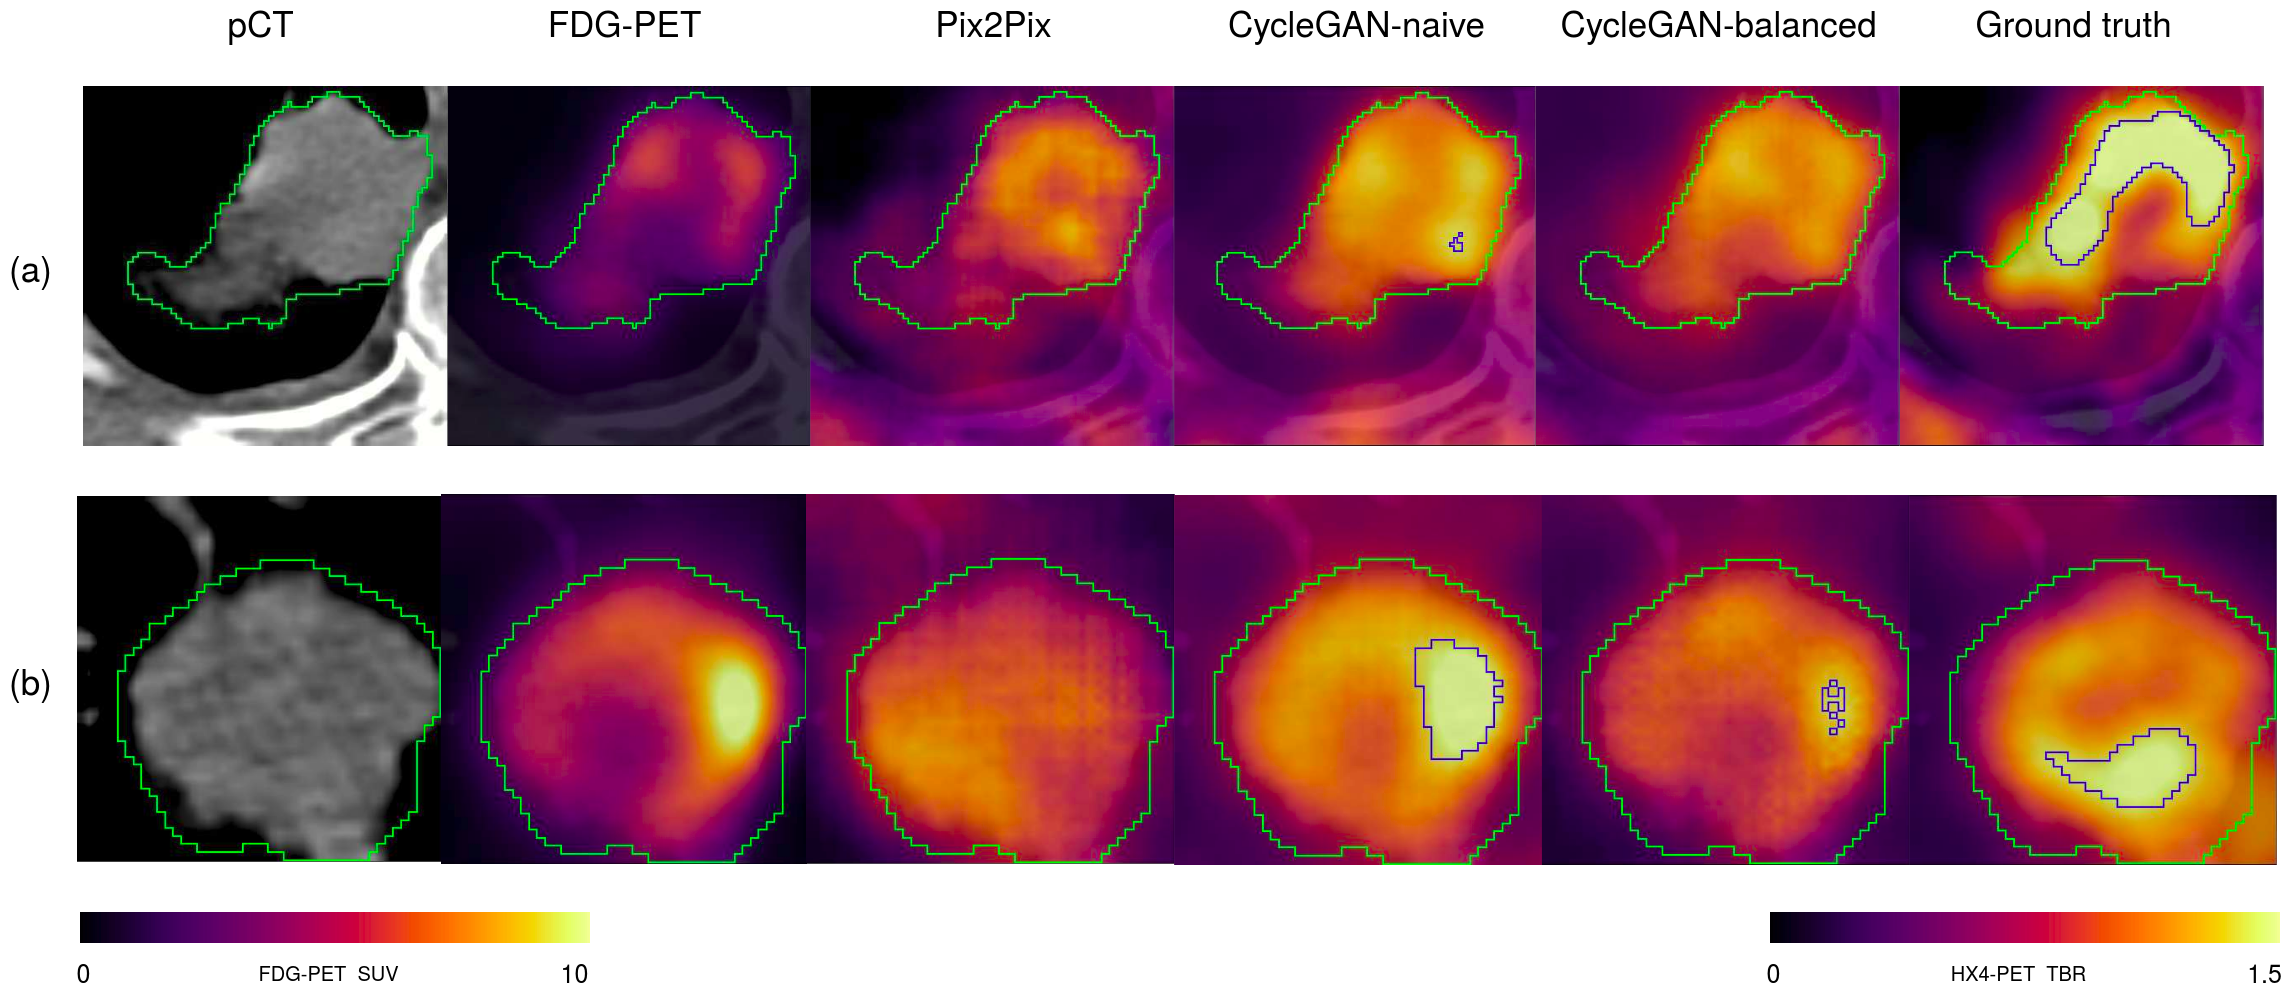
\includegraphics[width=\linewidth]{figures/Expt_3/hypoxia_viz.png}
    }
    \caption{Tumor hypoxia patterns generated by the models. All PET images are overlaid on the corresponding pCT. GTV is delineated with green contour, and the hypoxic region in each of three models' prediction and the ground truth is marked with blue contours. In both examples, Pix2Pix predictions didn't contain sufficiently intense regions, hence no hypoxic areas are seen segmented in these slices.}
    \label{fig:hypoxia_viz}
\end{figure}

One of the reasons Pix2Pix fails here appears to be related to its supervised training. The ground truth images contain registration errors that are more pronounced at the small scale in which this evaluation is performed. The fine hypoxia patterns in the ground truth, including those within the tumor, might have shifted post-registration causing misalignment with the CT and FDG-PET features, thereby inducing noise in the paired training data. Therefore, although the Pix2Pix model could produce synthetic hypoxia images of an overall higher quality, these images reveal large inaccuracies when examined at the scale of the tumor.
In case of the two CycleGANs, the tumor hypoxia patterns matched the spatial pattern of FDG uptake suggesting that the models learned to excessively depend on FDG-PET features. Another reason for poor clinical performance of all three models might be the small size of the training dataset. Even when using a patch-based training approach, the number of sufficiently varied training samples was very low. 

\chapter{Discussion}
\label{Discussion}

% Research qs were answered
In experiments \ref{Expt_1} and \ref{Expt_2}, we observe that the paired Pix2Pix approach can generate higher quality images as compared to unpaired CycleGAN, although at the cost of acquiring and preparing the ground truth images. Among the two CycleGAN systems, CycleGAN-balanced was able to circumvent the non-invertibility issue of CycleGAN-naive due to its design modification, and produced better results as indicated by both quantitative and qualitative analyses. Our quantitative evaluation of the synthetic HX4-PET images involved using a set of six metrics, of which three -- MSE, MAE, and PSNR -- measure the voxel-level accuracy of the synthetic images with respect to the ground truth, whereas the remaining three -- SSIM, NMI, and histogram distance -- account for the fidelity of image structure and statistics. Furthermore, each metric has its unique property and since the ``quality" of an image is a multifaceted attribute, using a population of such metrics for image assessment can capture the image quality more effectively as compared to using a subset of them. We thereby address our first research question. In \ref{cycelgan_convergence}, we perform an analysis of CycleGAN training losses over the training period and observe that the CycleGAN-balanced model was more stable and displayed better convergence properties as opposed to the CycleGAN-naive model, which diverged away from its objectives. The validation metrics collectively reflected similar trends as the convergence parameters while also being informative about model generalizability, thereby answering our third research question. Finally, through experiment \ref{Expt_3}, we address our second research question by identifying and performing clinically relevant downstream tasks to determine the clinical value of our synthetic HX4-PET images. Tumor hypoxia measurement derived from synthetic images from Pix2Pix showed remarkably poor accuracy compared with the two CycleGANs. While a majority of the tumors in the synthetic images produced by the CycleGAN models were classified correctly, the classification rate in Pix2Pix predictions is lower. However, as indicated by a poor segmentation score, none of the models could predict accurately the spatial distribution of high hypoxia. The primary reason could be the lack of sufficient training data, and the second reason, specifically for Pix2Pix, could be the noise in its supervision signal caused due to imperfect ground truth images. We believe that given sufficient training data, unpaired models like CycleGAN, especially the modified version of it, could be more suitable for the HX4-PET synthesis task. As supplementary material, we make available the \textit{WandB} training reports for the depth-estimation task (experiment \ref{Expt_1}) \footnote{Training report for the depth-estimation task: \url{https://bit.ly/3x452Qi}} and the HX4-PET synthesis task (experiment \ref{Expt_2}) \footnote{Training report for the HX4-PET synthesis task: \url{https://bit.ly/35Y8dx2}} which include training losses, validation metrics and intermediate outputs of the models.

% Some limitations, and opportunities for future work (stuff to do after thesis):
%   1. Dataset size -- larger training set to train better models, larger validation set to test properly
%   2. CycleGANs appeared to focus more on FDG features. Would be nice to see through an ablation study whether or not they really use CT features. One way to do this is taking the same trained models, turning off the CT signal in their input and performing inference.
%   3. With metrics - Need to consult more theoretical literature to understand their mathematical properties. This would allow choosing better and more diverse metrics to use and evaluate with the voting method.
%   4. Turing test
There are several limitations of this thesis that can provide opportunities for future work. First, the small size of our Maastro Lung HX4-PET dataset was a serious limitation on model training and validation. A larger training dataset would allow training better translation models and a sufficiently large and diverse validation dataset would enable more effective evaluation of the models. Second, it was observed that both the CycleGAN models predicted tumor hypoxia patterns that closely resembled the FDG uptake signatures rather than the actual spatial distribution of hypoxia. The models might have learned to heavily rely on FDG-PET features while ignoring CT information. It would be interesting to verify this by performing an ablation study on these models. This could be conducted, for instance, by performing inference with the fully trained models with the CT signal set to zero value and observing the generator outputs. Third, the quality assessment of the synthetic HX4-PET images was performed using a set of six general-purpose image quality and similarity metrics that were logically chosen. However, this portfolio of evaluation metrics can be improved. It would be valuable to consult theoretical literature on image metrics and understand in a greater depth their mathematical properties. This would help in selecting more suitable and diverse metrics thereby improving the comprehensiveness of image assessment. Fourth, as an extension of the simple automated clinical evaluation performed in experiment \ref{Expt_3}, a version of the Turing test can be performed by presenting the synthetic HX4-PET images to a radiation oncologist, with a certain clinically relevant goal, for instance, determining the prognostic value of the synthetic images. 


% Fine tuning stuff (questionable. don't include)
% Second, the Pix2Pix model failed in accurately predicting tumor hypoxia and produced high-frequency noise patterns in the tumor region, although its synthetic HX4-PET images were of an overall high quality. In addition to the registration-related issues, this failure can also be attributed to model training. In addition to using a larger training dataset as a possible solution to reducing these artifacts, it would be interesting to investigate into \textit{fine tuning} the trained Pix2Pix model using the existing dataset. This could be performed, for instance, by first using a patch-sampling strategy that focuses more on the tumor vicinity. Then, the weights of the Pix2Pix generator's encoder (which is its feature extractor) could be frozen while updating only its decoder (which is its image synthesizer). The intuition behind this is that, in doing so, the noise patterns can potentially be reduced since they caused during the upsampling operations used the decoder path, and that this by learning better upsampling kernels


% Expt 3 stuff (need this? probably not)
% We argue that although none of our models' synthetic HX4-PET was clinically satisfactory, paired translation approaches such as Pix2Pix that assume voxel-wise alignment are bound to produce inaccuracies in their images at a scale of the tumor.
% In our dataset, HX4-PET scans for all patient were acquired on a different day from FDG-PET and pCT acquisition. A problem with tumor hypoxia is the fact that the hypoxic region has a tendency to change over time, even over a period of hours [cite ...]. Zegers et al. \cite{zegers2013hypoxia} raise this argument to explain the relatively low \textit{voxel-level} correlation they observed between FDG-PET and HX4-PET SUV values despite a significant correlation on \textit{tumor-level} properties between the two modalities. It is possible that in our data, the state of the tumor captured by FDG-PET/pCT might not correspond perfectly to its state captured by HX4-PET. In such a case, even if the HX4-PET image were to be perfectly registered over pCT and FDG-PET, a supervised method that assumes voxel-level correspondence would be less effective, to say the least. In this view, it could then be possible that the hypoxia patterns predicted by the CycleGANs, although not matching the ground truth, might reflect the ``actual" hypoxia distribution.
\chapter{Conclusion}
\label{Conclusion}

In this work, we formulated the problem of predicting hypoxia from FDG-PET and CT scans as image-to-image translation and investigated image translation GANs for synthesizing full HX4-PET images from the multimodal input. Using the paired Pix2Pix and the unpaired CycleGAN, we observed that the paired approach produces superior quality images both in our simulated translation task and in the HX4-PET synthesis task. We argued that the naive application of CycleGAN to the HX4-PET synthesis task has a conceptual flaw related to non-invertibility of the inter-domain mappings, and proposed an alternative strategy to circumvent this problem while still relying on unpaired training data. This modified CycleGAN system showed substantial performance improvement over the default CycleGAN in terms of image quality. To assess the quality of the synthetic HX4-PET images in a comprehensive manner, we constructed a set of six measures of image quality and image similarity that measure broadly two different aspects of the images -- voxel-wise accuracy and (local and global) image statistics. A systematic visual inspection of the synthetic HX4-PET images validated the assessment of these metrics and also revealed common failure modes for each model. Images from Pix2Pix contained, on average, the least amount of degradation and artifacts, although they suffered from structural breaks in specific areas. These faults can be attributed to the supervised training of Pix2Pix which used ground truth images containing registration imperfections. Despite the clear image-quality-based performance differences across the three image translation models, the clinical evaluation of their synthetic images conducted via tumor hypoxia quantification tasks produced mixed and inconclusive results. These results were overall unsatisfactory indicating the insufficiency of the models in meeting the clinical requirements. The potential for clinical implementation of these image translation methods needs to be further investigated using larger and more diverse training and validation datasets. Between the paired and unpaired translation approaches, the latter could be more suitable due to their considerably more lenient data requirements and their lack of direct dependence on spatially aligned ground truth images that makes them immune to issues caused by misaligned training data.

\bibliographystyle{unsrt}
\bibliography{Bibliography}
\end{document}
